%%%%%%%%%%%%%%%%%%%%%%%%%%%%%%%%%%%%%%%%%%%%%%%%%%%%%%%%%%%%%%%
%% OXFORD THESIS TEMPLATE

% Use this template to produce a standard thesis that meets the Oxford University requirements for DPhil submission
%
% Originally by Keith A. Gillow (gillow@maths.ox.ac.uk), 1997
% Modified by Sam Evans (sam@samuelevansresearch.org), 2007
% Modified by John McManigle (john@oxfordechoes.com), 2015
% Modified by Ulrik Lyngs (ulrik.lyngs@cs.ox.ac.uk), 2018-, for use with R Markdown
%
% Ulrik Lyngs, 25 Nov 2018: Following John McManigle, broad permissions are granted to use, modify, and distribute this software
% as specified in the MIT License included in this distribution's LICENSE file.
%
% John commented this file extensively, so read through to see how to use the various options.  Remember that in LaTeX,
% any line starting with a % is NOT executed.  Several places below, you have a choice of which line to use
% out of multiple options (eg draft vs final, for PDF vs for binding, etc.)  When you pick one, add a % to the beginning of
% the lines you don't want.


%%%%% PAGE LAYOUT
% The most common choices should be below.  You can also do other things, like replacing "a4paper" with "letterpaper", etc.

% This one formats for two-sided binding (ie left and right pages have mirror margins; blank pages inserted where needed):
%\documentclass[a4paper,twoside]{templates/ociamthesis}
% This one formats for one-sided binding (ie left margin > right margin; no extra blank pages):
%\documentclass[a4paper]{ociamthesis}
% This one formats for PDF output (ie equal margins, no extra blank pages):
%\documentclass[a4paper,nobind]{templates/ociamthesis}

% As you can see from the uncommented line below, oxforddown template uses the a4paper size, 
% and passes in the binding option from the YAML header in index.Rmd:
\documentclass[a4paper, nobind]{templates/ociamthesis}


%%%%% ADDING LATEX PACKAGES
% add hyperref package with options from YAML %
\usepackage[pdfpagelabels]{hyperref}
% change the default coloring of links to something sensible
\usepackage{xcolor}

\definecolor{mylinkcolor}{RGB}{0,0,139}
\definecolor{myurlcolor}{RGB}{0,0,139}
\definecolor{mycitecolor}{RGB}{0,33,71}

\hypersetup{
  hidelinks,
  colorlinks,
  linktocpage=true,
  linkcolor=mylinkcolor,
  urlcolor=myurlcolor,
  citecolor=mycitecolor
}



% add float package to allow manual control of figure positioning %
\usepackage{float}

% enable strikethrough
\usepackage[normalem]{ulem}

% use soul package for correction highlighting
\usepackage{color, soul}
\definecolor{correctioncolor}{HTML}{CCCCFF}
\sethlcolor{correctioncolor}
\newcommand{\ctext}[3][RGB]{%
  \begingroup
  \definecolor{hlcolor}{#1}{#2}\sethlcolor{hlcolor}%
  \hl{#3}%
  \endgroup
}
\soulregister\ref7
\soulregister\cite7
\soulregister\autocite7
\soulregister\textcite7
\soulregister\pageref7

%%%%% FIXING / ADDING THINGS THAT'S SPECIAL TO R MARKDOWN'S USE OF LATEX TEMPLATES
% pandoc puts lists in 'tightlist' command when no space between bullet points in Rmd file,
% so we add this command to the template
\providecommand{\tightlist}{%
  \setlength{\itemsep}{0pt}\setlength{\parskip}{0pt}}
 
% UL 1 Dec 2018, fix to include code in shaded environments

% User-included things with header_includes or in_header will appear here
% kableExtra packages will appear here if you use library(kableExtra)
\usepackage{booktabs}
\usepackage{longtable}
\usepackage{array}
\usepackage{multirow}
\usepackage{wrapfig}
\usepackage{float}
\usepackage{colortbl}
\usepackage{pdflscape}
\usepackage{tabu}
\usepackage{threeparttable}
\usepackage{threeparttablex}
\usepackage[normalem]{ulem}
\usepackage{makecell}
\usepackage{xcolor}


%UL set section header spacing
\usepackage{titlesec}
% 
\titlespacing\subsubsection{0pt}{24pt plus 4pt minus 2pt}{0pt plus 2pt minus 2pt}


%UL set whitespace around verbatim environments
\usepackage{etoolbox}
\makeatletter
\preto{\@verbatim}{\topsep=0pt \partopsep=0pt }
\makeatother



%%%%%%% PAGE HEADERS AND FOOTERS %%%%%%%%%
\usepackage{fancyhdr}
\setlength{\headheight}{15pt}
\fancyhf{} % clear the header and footers
\pagestyle{fancy}
\renewcommand{\chaptermark}[1]{\markboth{\thechapter. #1}{\thechapter. #1}}
\renewcommand{\sectionmark}[1]{\markright{\thesection. #1}} 
\renewcommand{\headrulewidth}{0pt}

\fancyhead[LO]{\emph{\leftmark}} 
\fancyhead[RE]{\emph{\rightmark}} 

% UL page number position 
\fancyfoot[C]{\emph{\thepage}} %regular pages
\fancypagestyle{plain}{\fancyhf{}\fancyfoot[C]{\emph{\thepage}}} %chapter pages

% JEM fix header on cleared pages for openright
\def\cleardoublepage{\clearpage\if@twoside \ifodd\c@page\else
   \hbox{}
   \fancyfoot[C]{}
   \newpage
   \if@twocolumn\hbox{}\newpage
   \fi
   \fancyhead[LO]{\emph{\leftmark}} 
   \fancyhead[RE]{\emph{\rightmark}} 
   \fi\fi}


%%%%% SELECT YOUR DRAFT OPTIONS
% This adds a "DRAFT" footer to every normal page.  (The first page of each chapter is not a "normal" page.)

% IP feb 2021: option to include line numbers in PDF

% for line wrapping in code blocks
\usepackage{fvextra}
\DefineVerbatimEnvironment{Highlighting}{Verbatim}{breaklines,commandchars=\\\{\}}

% This highlights (in blue) corrections marked with (for words) \mccorrect{blah} or (for whole
% paragraphs) \begin{mccorrection} . . . \end{mccorrection}.  This can be useful for sending a PDF of
% your corrected thesis to your examiners for review.  Turn it off, and the blue disappears.
\correctionstrue


%%%%% BIBLIOGRAPHY SETUP
% Note that your bibliography will require some tweaking depending on your department, preferred format, etc.
% If you've not used LaTeX before, I recommend reading a little about biblatex/biber and getting started with it.
% If you're already a LaTeX pro and are used to natbib or something, modify as necessary.
% Either way, you'll have to choose and configure an appropriate bibliography format...


\usepackage[style=authoryear, sorting=nyt, backend=biber, maxcitenames=2, useprefix, doi=true, isbn=false, uniquename=false]{biblatex}
\newcommand*{\bibtitle}{Works Cited}

\addbibresource{bibliography/library.bib}
\addbibresource{bibliography/additional-references.bib}


% This makes the bibliography left-aligned (not 'justified') and slightly smaller font.
\renewcommand*{\bibfont}{\raggedright\small}


% Uncomment this if you want equation numbers per section (2.3.12), instead of per chapter (2.18):
%\numberwithin{equation}{subsection}


%%%%% THESIS / TITLE PAGE INFORMATION
% Everybody needs to complete the following:
\title{\texttt{oxforddown}:\\
An Oxford University Thesis\\
Template for R Markdown}
\author{Keana Richards}
\college{University of Pennsylvania}

% Master's candidates who require the alternate title page (with candidate number and word count)
% must also un-comment and complete the following three lines:

% Uncomment the following line if your degree also includes exams (eg most masters):
%\renewcommand{\submittedtext}{Submitted in partial completion of the}
% Your full degree name.  (But remember that DPhils aren't "in" anything.  They're just DPhils.)
\degree{Doctor of Philosophy}
% Term and year of submission, or date if your board requires (eg most masters)
\degreedate{Michaelmas 2018}


%%%%% YOUR OWN PERSONAL MACROS
% This is a good place to dump your own LaTeX macros as they come up.

% To make text superscripts shortcuts
	\renewcommand{\th}{\textsuperscript{th}} % ex: I won 4\th place
	\newcommand{\nd}{\textsuperscript{nd}}
	\renewcommand{\st}{\textsuperscript{st}}
	\newcommand{\rd}{\textsuperscript{rd}}

%%%%% THE ACTUAL DOCUMENT STARTS HERE
\begin{document}

%%%%% CHOOSE YOUR LINE SPACING HERE
% This is the official option.  Use it for your submission copy and library copy:
\setlength{\textbaselineskip}{22pt plus2pt}
% This is closer spacing (about 1.5-spaced) that you might prefer for your personal copies:
%\setlength{\textbaselineskip}{18pt plus2pt minus1pt}

% You can set the spacing here for the roman-numbered pages (acknowledgements, table of contents, etc.)
\setlength{\frontmatterbaselineskip}{17pt plus1pt minus1pt}

% UL: You can set the line and paragraph spacing here for the separate abstract page to be handed in to Examination schools
\setlength{\abstractseparatelineskip}{13pt plus1pt minus1pt}
\setlength{\abstractseparateparskip}{0pt plus 1pt}

% UL: You can set the general paragraph spacing here - I've set it to 2pt (was 0) so
% it's less claustrophobic
\setlength{\parskip}{2pt plus 1pt}

%
% Oxford University logo on title page
%
\def\crest{{
\includegraphics[width=5cm]{templates/beltcrest.pdf}}}
\renewcommand{\university}{University of Pennsylvania}
\renewcommand{\submittedtext}{A thesis submitted for the degree of}


% Leave this line alone; it gets things started for the real document.
\setlength{\baselineskip}{\textbaselineskip}


%%%%% CHOOSE YOUR SECTION NUMBERING DEPTH HERE
% You have two choices.  First, how far down are sections numbered?  (Below that, they're named but
% don't get numbers.)  Second, what level of section appears in the table of contents?  These don't have
% to match: you can have numbered sections that don't show up in the ToC, or unnumbered sections that
% do.  Throughout, 0 = chapter; 1 = section; 2 = subsection; 3 = subsubsection, 4 = paragraph...

% The level that gets a number:
\setcounter{secnumdepth}{2}
% The level that shows up in the ToC:
\setcounter{tocdepth}{1}


%%%%% ABSTRACT SEPARATE
% This is used to create the separate, one-page abstract that you are required to hand into the Exam
% Schools.  You can comment it out to generate a PDF for printing or whatnot.

% JEM: Pages are roman numbered from here, though page numbers are invisible until ToC.  This is in
% keeping with most typesetting conventions.
\begin{romanpages}

% Title page is created here
\maketitle

%%%%% DEDICATION -- If you'd like one, un-comment the following.
%%%%% %%%%% \begin{dedication}
%%%%%  For my mom
%%%%% \end{dedication}
%%%%% 
%%%%% ACKNOWLEDGEMENTS -- Nothing to do here except comment out if you don't want it.

\addcontentsline{toc}{chapter}{Acknowledgements}
\renewcommand{\numberstyleacks}{plain}
\renewcommand{\numberstyleabstract}{plain}


\begin{acknowledgements}
 	This is where you will normally thank your advisor, colleagues, family and friends, as well as funding and institutional support. In our case, we will give our praises to the people who developed the ideas and tools that allow us to push open science a little step forward by writing plain-text, transparent, and reproducible theses in R Markdown.

  We must be grateful to John Gruber for inventing the original version of Markdown, to John MacFarlane for creating Pandoc (\url{http://pandoc.org}) which converts Markdown to a large number of output formats, and to Yihui Xie for creating \texttt{knitr} which introduced R Markdown as a way of embedding code in Markdown documents, and \texttt{bookdown} which added tools for technical and longer-form writing.

  Special thanks to \href{http://chester.rbind.io}{Chester Ismay}, who created the \texttt{thesisdown} package that helped many a PhD student write their theses in R Markdown. And a very special thanks to John McManigle, whose adaption of Sam Evans' adaptation of Keith Gillow's original maths template for writing an Oxford University DPhil thesis in LaTeX provided the template that I in turn adapted for R Markdown.

  Finally, profuse thanks to JJ Allaire, the founder and CEO of \href{http://rstudio.com}{RStudio}, and Hadley Wickham, the mastermind of the tidyverse without whom we'd all just given up and done data science in Python instead. Thanks for making data science easier, more accessible, and more fun for us all.

  \begin{flushright}
  Ulrik Lyngs \\
  Linacre College, Oxford \\
  2 December 2018
  \end{flushright}
\end{acknowledgements}



%%%%% ABSTRACT -- Nothing to do here except comment out if you don't want it.

\addcontentsline{toc}{chapter}{ABSTRACT}
\renewcommand{\numberstyleabstract}{plain}

\renewcommand{\abstracttitle}{ABSTRACT}
\begin{abstract}
	This \emph{R Markdown} template is for writing an Oxford University thesis. The template is built using Yihui Xie's \texttt{bookdown} package, with heavy inspiration from Chester Ismay's \texttt{thesisdown} and the \texttt{OxThesis} \LaTeX~template (most recently adapted by John McManigle).

 This template's sample content include illustrations of how to write a thesis in R Markdown, and largely follows the structure from \href{https://ulyngs.github.io/rmarkdown-workshop-2019/}{this R Markdown workshop}.

 Congratulations for taking a step further into the lands of open, reproducible science by writing your thesis using a tool that allows you to transparently include tables and dynamically generated plots directly from the underlying data. Hip hooray!
\end{abstract}


%%%%% MINI TABLES
% This lays the groundwork for per-chapter, mini tables of contents.  Comment the following line
% (and remove \minitoc from the chapter files) if you don't want this.  Un-comment either of the
% next two lines if you want a per-chapter list of figures or tables.
  \dominitoc % include a mini table of contents

% This aligns the bottom of the text of each page.  It generally makes things look better.
\flushbottom

% This is where the whole-document ToC appears:
\tableofcontents

\listoffigures
	\mtcaddchapter
  	% \mtcaddchapter is needed when adding a non-chapter (but chapter-like) entity to avoid confusing minitoc

% Uncomment to generate a list of tables:
\listoftables
  \mtcaddchapter
%%%%% LIST OF ABBREVIATIONS
% This example includes a list of abbreviations.  Look at text/abbreviations.tex to see how that file is
% formatted.  The template can handle any kind of list though, so this might be a good place for a
% glossary, etc.

% The Roman pages, like the Roman Empire, must come to its inevitable close.
\end{romanpages}

%%%%% CHAPTERS
% Add or remove any chapters you'd like here, by file name (excluding '.tex'):
\flushbottom

% all your chapters and appendices will appear here
\hypertarget{chapter-1}{%
\chapter{Chapter 1}\label{chapter-1}}

\hypertarget{introduction}{%
\section{Introduction}\label{introduction}}

Women have surpassed men in education outcomes, like college attendance and graduation rates \autocite{Blau2017,Goldin2006,Stoet2014}, but continue to be underrepresented in top management positions in nearly all sectors \autocite{Bertrand2001}. And, a sizable gender gap still persists worldwide \autocite{Blau2017}. Traditional economic variables, such as household division of labor and discrimination, account for some, but not all, of these disparities \autocite{Blau2017}. As such, researchers have begun to consider psychological gender differences, including the predilection for competition, as means of understanding persistent gender gaps in labor market outcomes \autocite[for review, see][]{Niederle2011}.

Research suggests women are, on average, less competitive than men (for review, see \textcite{Niederle2011}). Seminal work on gender differences in competitiveness operationalized competitiveness as the choice of a tournament payment scheme, that reaps potentially higher earnings but requires outperforming an opponent, over a piece-rate scheme, where participants are paid per unit of work they produce \autocite{Niederle2007}. In this paradigm, women are less likely to enter tournaments while completing mathematical problems, even when they would have earned more by competing \autocite{Niederle2007}. Numerous conceptual replications over the past 15 years suggests that the gender difference in willingness to compete is robust \autocites[see][ for review]{Niederle2011,Niederle2017a,Niederle2017b}. Notably, this effect has been replicated in diverse populations (e.g., across age groups and cultures) \autocite{Apicella2015,Buser2014,Sutter2016,Andersen2013,Buser2017b,Sutter2010,Dreber2014,Mayr2012} and with a diverse set of tasks \autocite{Apicella2015,Saccardo2018,Bjorvatn2016,Sutter2015,Frick2011,Samek2019}. Importantly, this laboratory measure of competitiveness predicts labor market outcomes, including education choices \autocite{Buser2014,Zhang2012}, entrepreneurial decisions {[}e.g., investment, employment; \textcite{Berge2015}{]}, and earnings \autocite{Reuben2015}. In other words, competitive preferences may contribute to the gender gap in labor market outcomes \autocite{Blau2017}. Thus, understanding why men and women differ in levels of competitiveness and whether interventions exist that can reduce or eliminate the difference may be key for solving the pernicious gender gaps in the labor market.

Both confidence and risk attitudes have been implicated in driving gender differences in willingness to compete \autocite{Niederle2011,Veldhuizen2017}. However, the extent to which confidence and risk attitudes account for the gender difference in willingness to compete is debated. The seminal research in this literature suggests that confidence and risk attitude do not completely explain gender differences in competitiveness, since there remained a residual gap after controlling for these factors \autocite{Niederle2007}. As a result, the unexplained component of the original gender effect was taken as evidence of a distinct ``competitiveness'' trait, separate from risk attitude and confidence \autocite{Niederle2007,Niederle2011}. Conversely, recent work correcting for measurement error \autocite{Gillen2019} and using experimental techniques to isolate the effects of the competitiveness trait \autocite{Veldhuizen2017} suggests that risk attitudes and confidence can fully explain the gender gap in the choice to compete.

Regardless of whether competitiveness is a ``stand-alone'' trait, it is clear that both confidence and risk attitude influence how men and women react to competitions. For instance, even in the original study by Niederle and Vesterlund (2007), 27\% of the gender gap in tournament entry was explained by men being more overconfident than women about their relative performance on the task. As such, interventions designed to increase women's confidence and decrease their perceptions of risk and uncertainty in competitive contexts may help reduce the gender gap in competitiveness.

Confidence is conceptualized as the accuracy of one's perceived performance or ability on a task \autocite{Beyer1997}. Within the literature on the gender gap in competitiveness, confidence is operationalized as the belief about one's relative performance during a competition, where individuals who have inaccurately high (low) ratings of their performance are deemed overconfident (underconfident). If an individual does not believe their performance is higher than the individuals they are competing against, they are unlikely to make the decision to compete for fear of missing the opportunity to earn money.

While most individuals are overconfident \autocite{Alicke2013,Dunning2004b}, there is ample research to suggest that women are less (over)confident on average than men across a number of domains \autocite{Mobius2011,Niederle2011,Croson2009,Lundeberg1994,Niederle2007,Bertrand2010a,Beyer1990,Beyer1997,Jakobsson2013}. Because women are less overconfident, they compete less often than they should, given their actual ability \autocite{Niederle2007}. Confidence too may help explain why, in some situations, the gender gap in competitiveness may be reduced or eliminated. For instance, women tend to compete more when tasks are female-typed or gender-neutral \autocite{Iriberri2017,Boschini2014,Boschini2019,Apicella2015,Grosse2010,Gunther2010,Dreber2014,Dreber2011,Shurchkov2012}, when they are facing other female opponents \autocite{DattaGupta2013,Booth2012}, or when competing against themselves {[}\textcite{Apicella2017a}; insert cites from here: \url{https://www.sciencedirect.com/science/article/pii/S0014292121001306?casa_token=-TmBt5-XsdMAAAAA:g-SfgLpuWqjY1lBKbp1xzp0lhj9Ibl9z6DCm-D3Xf6vRHGHHK_x_1ABc5Erf25FjdZ2Uf1NLpn4} - aka = Bönte et al., 2017; Klinowski, 2017; Carpenter et al., 2018; Apicella et al., 2020; Demiral and Mollerstrom, 2020{]}. For example, Apicella et al.~(2017) document a gender difference in confidence when women and men are competing against other individuals, but not when they are competing against themselves (i.e., their own past performance). There are several non-mutually exclusive and potentially interacting explanations that could account for women's relatively lower (over)confidence, including differences in performance or ability, experience, innate psychological differences, and stereotype threat \autocite{Steele1997,Spencer1999,Spencer2016}. In the latter case, for instance, women may decide to forgo competitions because they either believe negative stereotypes about their ability to perform certain tasks, or because stereotypes provoke enough anxiety to reduce confidence \autocite{Gunther2010,Grosse2010,Iriberri2017,Shurchkov2012,Burow2017}. Taken together, this body of research suggests that interventions designed to increase confidence in women, may embolden them to compete more.

A second variable that has been identified as a possible explanation for gender differences in competitiveness is risk attitude, typically construed as the preference for a certain gain over a gamble, even if the gamble has an equal or greater monetary expectation \autocite{Kahneman1982}. Researchers investigating gender differences in risk attitudes find that men are typically more risk-seeking than women \autocite{Eckel2008,Charness2012,Croson2009,Bertrand2010a}, including in hunter-gatherers \autocite{Apicella2017}, but see \autocite{Harrison2007} for an exception. While most studies report a gender difference, the difference appears to be small to medium \autocite{Filippin2016} and culturally-dependent {[}Anderson, et al.~2013; \textcite{Gneezy2009}{]}.

Competitive payment schemes are inherently riskier than piece-rate payment schemes because the variance in returns is greater. With piece-rate payment schemes, individuals are guaranteed a certain amount for every unit they produce. Moreover, there typically exists uncertainty in competitions since one's relative performance is unknown \autocite{Niederle2011}. Indeed, some of the gender gap in competitiveness is explained by men and women's differing risk attitudes \autocite{Niederle2011}. In fact, some recent work suggests that nearly 30\% of the gender gap in competitive choices can be explained by risk attitude \autocite{Gillen2019,Veldhuizen2017}.

In the current study, we examine whether and how preparation may influence willingness to compete. Preparation or training on a task may increase one's confidence \autocite{Gist1992,Schunk1981,Schunk1982,Usher2008}, since people usually are able to observe an improvement in their performance over time. \textcite{Lent1996} found that college students listed past accomplishments as the most influential factor in determining their confidence. Moreover, research directly comparing the effects of mastery experiences (via preparation), vicarious experiences (e.g., watching others perform a task), and a control treatment without any intervention on confidence, found that mastery increased confidence significantly more than vicarious experiences and the control treatment \autocite{Bandura1977a}. Other research suggests that men and women's confidence is similar in domains in which they have expertise, but the confidence gap emerges when it is assessed in less knowledgeable domains \autocite{Sarsons2016}. This suggests that gaining expertise, perhaps through practicing, may selectively boost women's confidence. \textcite{Roll2011} found that practicing mathematics problems, using an intelligent tutoring system, significantly decreases under-confidence but has no effect on rates of over-confidence. This too suggests that practicing may preferentially benefit women who are more likely than men to be underconfident. That said, if practicing only helps with under-confidence, when most people, including women, are overconfident, then its application may be limited.

Preparation, and the feelings of preparedness or self-efficacy that follow, may also decrease the perceived riskiness of competitions. With increased self-efficacy, individuals may believe they can reduce risk or overcome adversity. Surprisingly little work has explored how preparation impacts men's and women's risk attitudes. However, some experimental work suggests that manipulating perceived competence on a task by giving participants positive feedback about their performance on a task can lead to significantly more risk-taking behavior \autocite{Krueger1994}. The researchers were able to rule out the role of mood in driving the results by giving some participants positive feedback on one task and negative feedback on another. For these participants, risk-taking increased in the positive feedback condition and decreased in the negative feedback condition. Interestingly, \textcite{Gysler2002} find that knowledge -- in this case, understanding of financial markets -- and confidence in that knowledge, negatively correlate with women's risk aversion, but positively correlate with men's risk aversion. This suggests that preparation may disproportionately increase risk-taking in women. Finally, there is evidence that risk attitudes play a greater role in predicting decisions to compete when individuals are competing against other individuals, rather than themselves (i.e., their own past performance), possibly because there is more uncertainty in estimating an opponent's ability versus one's own ability \autocite{Apicella2017a}.

Surprisingly, little work has explored how preparation impacts men and women's confidence, risk attitudes, or their willingness to compete. We know of only one study that has explored how a delaying a competition, and in some cases, offering an opportunity to study, affects decisions to compete. In a working paper, \textcite{Charness2021} examine whether gender gap entry rates change when a future opportunity to study for the task is made available. The authors hypothesized that women would be more likely to compete when there is an opportunity to study for the task. Contrary to their prediction, the authors found that providing an option to study leads to directionally more male entries into future planned tournaments and directionally less female entries into these tournaments, resulting in a significant gender gap. However, this gap was only present during the initial, provisional sign-up period. When the actual choice was made later -- sometime between one-five days -- the gender difference disappeared. Of those men who returned to complete the study, some switched into the non-competitive payment scheme. The authors suggest that the results may be explained by men being overly confident in their future selves' resolve to study.

We similarly examine the role of preparation on the gender differences in willingness to compete through three experiments. However, unlike \textcite{Charness2021}, we do not introduce a significant time delay in our studies. That is, experiments took place in a single session, thus minimizing any potential for gender differences in beliefs about future selves to affect our results.

In the first experiment, we test whether simply knowing that there will be an opportunity to prepare before performing a task affects the gender gap in willingness to compete. That is, we manipulate participants' knowledge of whether they will have time to prepare before they make their decision to compete. We anticipate that participants with this information would be more inclined to compete compared to participants without this information and that this effect would be stronger for women, who tend to be relatively less confident. Thus, we expected an interaction between gender and condition on the choice to compete, along with a main effect of condition. In the second experiment, we examined how actual preparation influences the decision to compete. That is, we manipulated whether participants were required to prepare before making the decision to compete. Again, we expected that women in the preparation condition would be especially inclined to compete. Finally, in experiment 3, we examine how an unlimited amount of preparation affects gender differences in the willingness to compete. Across all experiments, we measured gender differences in actual preparation after administering the treatment and eliciting preferences to compete. Finally, we monetarily incentivized participants in both studies to correctly predict which gender would prepare and compete more. The research design, hypotheses, measures and analyses were preregistered unless otherwise stated and all analyses were conducted in R statistical software (version 4.0.4).

\hypertarget{study-1}{%
\section{Study 1}\label{study-1}}

\hypertarget{methods}{%
\subsection{Methods}\label{methods}}

We recruited workers on Amazon Mechanical Turk for Study 1, and those who opted into the study had to pass several screening questions. Specifically, participants included in the paid portion of the study had to (i) identify their nationality as American and live in the United States, (ii) identify as a man or a woman, and (iii) be using a computer (rather than a phone or tablet). If they did not meet these criteria, they did not proceed to the paid portion of the study. Additionally, upon reviewing the data, we had reason to suspect that some participants completed the study more than once. Specifically, some participants had the same IP address, MTurk ID, and were of the same gender. When entries matched on all three identifiers, we included only the first entry and excluded all subsequent entries. The final sample consisted of 1056 participants (53.6\% women), with an average age of 37.74 (\emph{SD} = 13.19) years. 54 participants (53.7\% women) dropped out of the study before finishing and we use their data when available.

Participants were told they would be completing a multiplication task where they would be able to choose how they would be paid for their performance. We chose a multiplication task because we expect participants will improve with practice. Indeed, research suggests that rehearsing and recalling associative memories can speed up retrieval of those memories \autocite{Rundus1971}. The task involved solving problems from multiplication tables 1-12 as quickly as possible within a two-minute period. They were provided an example of a question with the correct response and had to answer three practice problems correctly to proceed, as a test of their comprehension. After completing the comprehension questions, participants were randomly assigned to either a ``knowledge of preparation'' condition or a control condition. Participants in the ``knowledge of preparation'' condition were presented the following text:

``There is an option to practice/study before completing the multiplication task that is available to all participants. If you take this opportunity to practice/study, we will provide you with materials that may help boost your performance in the multiplication task. You will have unlimited time to practice/study before completing the task. You can stop practicing/studying at any point.''

Participants assigned to the control condition simply proceeded without seeing this text. Then, all participants learned about the two possible payment schemes (either piece-rate or tournament) that they would have the option to choose from and had to correctly answer questions testing their comprehension of the payment schemes.

Under the piece-rate scheme participants were told that they would be paid \$.10 for every problem answered correctly. Under the tournament scheme, participants were told that they would be paid \$.20 for every problem they answered correctly, but only if they answered more questions correctly than a randomly assigned competitor. Participants in the experimental condition were reminded that they had the option to prepare before completing the task. The order of presentation of the tournament and piece-rate payment options was randomized for participants.

After choosing a payment scheme, participants in both conditions were given an opportunity to prepare before the multiplication task. If they chose to prepare, participants were presented with each multiplication table, 1 through 12, in sequential order. Each multiplication table provided products of numbers up to 12. Thus, participants could use the table to study. Additionally, participants were asked if they wanted to complete practice problems. If they said yes, participants were asked to solve all multiples in that table and could only proceed to the next table if they answered all the questions correctly.

Once they completed all practice questions for a given times table, they were shown the multiplication table again and were asked if they would like to continue solving problems from that table or move onto the next multiplication table. This process was repeated for each multiplication table. Thus, we had two measures of preparation behavior: the decision to practice and the total number of times participants completed each multiplication table. The decision to practice measure conceptually captures a participants' baseline willingness to prepare, before they know what the preparation will involve. Thereafter, the total number of preparation rounds reflects participants' willingness to repeatedly prepare.

Following the preparation portion of the study, participants moved on to the paid portion of the study. They were required to solve as many problems as possible in two minutes. After completion, participants were told how many problems they answered correctly and completed a series of incentivized follow-up questions, including confidence and perceptions of gender differences. For these measures, participants were told one of these questions would be selected for a possible bonus payment, and if they answered the selected question correctly, they would earn a bonus of \$.10. For the measure of confidence, participants were asked to correctly predict their relative performance compared to all other participants completing the task by indicating the decile of their score. Notably, the item was phrased so participants did not need to understand the word ``decile,'' but were asked instead: ``If my performance is compared to that of all participants that completed the task, I think my score was\ldots{}'' with the options for responses ranging from ``Better than all other participants'' to ``Better than none of the other participants'' with 10\% increments in between (e.g., ``Better than 50\% of participants''). Participants were also asked to correctly predict which gender 1) correctly solved more problems 2) spent more time practicing before completing the multiplication task, and 3) chose the tournament payment option more.

Finally, participants completed a measure of risk aversion, where they answered if they generally are willing to take risks or try to avoid taking risks \autocite{Dohmen2011} on a 10 point scale with 0 meaning participants are ``Not at all willing to take risks'' and 10 indicating participants are ``Very willing to take risks.'' To determine whether participants used additional tools to improve their performance on the task, we also asked participants about their use of calculators and perceptions of calculator use on the multiplication task. Neither of these measures was incentivized.

\hypertarget{results}{%
\subsection{Results}\label{results}}

An equal number of participants were assigned to both conditions (control= 50\%). Of the males who completed the study, 49.9\% were assigned to the control condition. Of the females who completed the study, 50.09\% were assigned to the control condition.

A minority of participants (15.41\%) chose to compete, contrary to previous data in this literature \autocite{Niederle2007}. Despite the small proportion of participants who chose to compete, we still replicate the gender gap in the choice to compete, where a greater share of men (19.59\%) compared to women (10.78\%) chose to compete. A logistic regression revealed that this gender difference in the choice to compete is significant, \(b = -0.73\), 95\% CI \([-1.23\), \(-0.24]\), \(z = -2.90\), \(p = .004\). Contrary to our predictions, we do not find evidence of a significant interaction between gender and condition on the decision to compete, \(b = 0.06\), 95\% CI \([-0.63\), \(0.76]\), \(z = 0.18\), \(p = .861\) (see Figure \ref{fig:s100}), suggesting that women in the knowledge of preparation condition were not uniquely more inclined to compete.

As hypothesized, women were 75.47\% more likely to take advantage of the opportunity to practice relative to men, \(b = 0.56\), 95\% CI \([0.31\), \(0.82]\), \(z = 4.37\), \(p < .001\), while controlling for the decision to compete (see Figure \ref{fig:s101}). As an exploratory analysis, we tested whether gender and the choice to compete interact to predict the choice to prepare, but did not find evidence for an interaction, \(b = 0.12\), 95\% CI \([-0.60\), \(0.86]\), \(z = 0.33\), \(p = .740\).

In further support of gender differences in preparation, women completed 87.79\% more rounds of preparation relative to men, \(b = 0.63\), 95\% CI \([0.46\), \(0.80]\), \(z = 7.32\), \(p < .001\) (see Figure \ref{fig:s102}). Thus, we have evidence that women prepare more both 1) before they know what the preparation entails and 2) after they have had the chance to experience the preparation. One can imagine that these would be driven by distinct psychological mechanisms, where 1) captures whether a person generally takes advantage of any opportunity to prepare, regardless of what it involves, while 2) measures a person's willingness to persist in their preparation, even after exerting effort previously during preparation. The fact that we find gender differences across two different forms of willingness to prepare suggests that the findings are robust. This gender difference aligned with participants' predictions about gender differences in preparation, where participants expected women, relative to men, to spend more time preparing for the multiplication task, \(\chi^2(1, n = 1056) = 15.67\), \(p < .001\) (see Figure \ref{fig:s103}), and in general, \(\chi^2(1, n = 1056) = 447.11\), \(p < .001\) (see Figure \ref{fig:s106}). One possible explanation for participants' predictions is that they expected men to outperform women on the task, which would lead women to compensate by preparing more. However, participants did not expect any gender differences in performance on the task, \(\chi^2(1, n = 1056) = 1.02\), \(p = .313\) (see Figure \ref{fig:s104}). Additionally, participants accurately predicted that women were less likely to choose to compete, \(\chi^2(1, n = 1056) = 716.24\), \(p < .001\) (see Figure \ref{fig:s105}), suggesting that they did not believe women prepare more because they were more likely to compete.

\hypertarget{study-2}{%
\section{Study 2}\label{study-2}}

\hypertarget{methods-1}{%
\subsection{Methods}\label{methods-1}}

Participants were recruited on Amazon Mechanical Turk using the same screening criteria as Study 1. Also, if participants had an identical IP address, MTurkID, and gender, we excluded their second response. The final sample consisted of 1088 participants (50.64\% women), with an average age of 38.54 (\emph{SD} = 12.5) years. 62 participants (51.61\% women) dropped out of the study before finishing.

As in Study 1, participants included in the study were told they would be completing a two-minute multiplication task (identical to the one used in Study 1) and would be able to choose a payment scheme for their performance. The instructions and payment per question were identical to Study 1. After being told about the rules for the multiplication task and passing the same comprehension questions used in Study 1, participants were assigned to either a preparation condition, where they were told they would complete several rounds of preparation before completing the multiplication task, or a control condition, where they were told they would complete several rounds of a counting task before continuing. Participants were randomly assigned to each condition. The participants in the preparation condition completed 12 rounds (one round per multiplication table), with 6 problems per round. The problems for each round were selected at random. Participants in the control condition were asked to complete 5 questions where they counted the number of zeros in a matrix of zeros and ones. After a 30-second break following completion of their respective tasks, all participants chose a payment scheme for the multiplication task, where the order of presentation was counterbalanced. That is, half of participants saw the tournament scheme presented as the first option and half saw the piece-rate payment scheme presented first.

After choosing a payment scheme, participants in both conditions had the option to spend (extra) time preparing for the multiplication task. Again, we had two measures of preparation behavior: the decision to practice and the total number of times participants completed the multiplication table. If they chose to prepare, participants were given two minutes to complete a randomly selected set of problems from all 12 multiplication tables. Once they finished the first two-minute preparation round, participants could opt into 4 more rounds of preparation, each two minutes long, before they moved on to the paid portion of the study.

Then, participants completed the paid multiplication task for two minutes. We included many of the same follow-up questions as in Study 1, including risk aversion, confidence, and perceptions of gender differences in preparation, competitiveness, and performance. Participants were incentivized to answer the questions about their confidence and perceptions of gender differences correctly, and were paid at the same rate as Study 1. We also asked participants if they wished they had more time to prepare for the multiplication task and included measures of their fatigue, field-specific ability beliefs, and interest in the multiplication task all on 1 (Strongly disagree) to 7 (Strongly agree) scales. For the fatigue scale, participants rated how fatigued and mentally exhausted they felt \autocite{Milyavskaya2018}. Participants indicated the degree to which they ``enjoyed completing the multiplication task'' for the interest scale \autocite{Milyavskaya2018}. Finally, to measure field-specific ability beliefs, we asked participants how much they perceived success in math depends on ability versus effort through six questions (e.g., ``If you want to succeed in math, hard work alone just won't cut it; you need to have an innate gift or talent'') \autocite{Meyer2015}.

\hypertarget{results-1}{%
\subsection{Results}\label{results-1}}

An equal number of participants were assigned to both conditions (control= 50.05\%). Of the males who completed the study, 50.09\% were assigned to the control condition and of the females who completed the study, 50\% were assigned to the control condition.

We replicated the effect of gender on the choice to compete: 19.18\% of men chose to compete compared to 13.43\% of women. However, we do not find evidence of a significant effect of condition on the choice to compete among women, \(b = -0.29\), 95\% CI \([-0.79\), \(0.21]\), \(z = -1.14\), \(p = .255\) (see Figure \ref{fig:s200}), contrary to our hypotheses.

Despite no evidence for the effect of condition on the choice to compete among women, we replicate the effects found in Study 1, where women were significantly more likely to prepare for the task, even after being forced to prepare in the preparation condition (see Figure \ref{fig:s204}). Women were 18.57\% more likely to take advantage of the opportunity to prepare relative to men \(b = 0.17\), 95\% CI \([0.00\), \(0.34]\), \(z = 1.99\), \(p = .047\), while controlling for the decision to compete (see Figure \ref{fig:s204}). Again, we find that these results align with participants' expectations, where they were significantly more likely to expect women to choose to prepare in general, \(\chi^2(1, n = 1088) = 513.72\), \(p < .001\) (see Figure \ref{fig:s203}), despite expecting men to choose to compete more often, \(\chi^2(1, n = 1088) = 580.69\), \(p < .001\) (see Figure \ref{fig:s202}) and expecting no gender differences in performance on the task, \(\chi^2(1, n = 1088) = 0.51\), \(p = .473\) (see Figure \ref{fig:s201}).

\hypertarget{discussion}{%
\section{Discussion}\label{discussion}}

\hypertarget{describing-goals-of-research-and-main-descriptive-findings}{%
\section{Describing goals of research and main descriptive findings}\label{describing-goals-of-research-and-main-descriptive-findings}}

Previous research suggests that women tend to be more risk-averse \autocite{Croson2009,Dohmen2011b,Eckel2008,Bertrand2010a} and less confident \autocite{Bertrand2010,Lundeberg1994,Mobius2011,Barber2001,Croson2009}, which affects their decisions to compete. Since confidence and risk attitudes may be affected by the opportunity to prepare, women may be more likely to compete when they have the opportunity to prepare before entering a competition. Through three experiments, we explored whether the opportunity to prepare affects gender differences in competitiveness and whether there are gender differences in willingness to prepare.

Within our design framework, we replicate the effect of gender on the choice to compete when gender is included as the only predictor in the model, but the gender difference in the choice to compete goes away when controlling for task score, risk, and confidence across all three studies (like apicella et al). There are a couple of possible reasons we do not consistently replicate the gender difference in competitiveness using our study design. There might be something unique about the task or online nature of the competition (eg like apicella study, insert other cites with similar designs) that leads us to find slightly different effects than the literature.

previous literature that uses online tasks:
\textcite{Charness2021} does not find evidence of a gender difference in competitiveness in gender-neutral task (aka counting zeros task). They suggest that gender gap in the choice to compete depends on the circumstances and beliefs.
\textcite{Apicella2020} does not find gender difference in competition
\textcite{Apicella2017} finds gender difference in competition

Though we do not consistently find evidence for the the gender difference in competitiveness when controlling for other predictors, we find evidence that gender consistently predicts risk and confidence across studies, replicating previous effects found within the literature {[}cites{]}. Next, we explored the effects of our preparation manipulations on the choice to compete across studies.

\hypertarget{summarizing-effects-of-preparation-condition-on-choice-to-compete}{%
\section{Summarizing effects of preparation condition on choice to compete}\label{summarizing-effects-of-preparation-condition-on-choice-to-compete}}

First, we find no evidence that preparation increases men or women's willingness to compete. In fact, in Study 3 we find that women in the control condition were significantly \emph{more} likely to compete than women in the control condition, despite believing that practicing helps performance on the main task both based on their behavior and their responses to the manipulation check question. We explored whether the unexpected effect in Study 3 was driven by increased perceptions of risk or reduced confidence when participants were assigned to the practice condition relative to the control condition, and did not find strong evidence for that possible explanation.

One possible reason women assigned to the preparation condition competed less is that they did not feel as though they were practicing as much as others, leading them to avoid the competition altogether because they expected to be at a disadvantage if they were to have chosen to compete. That is, even though they might choose to practice multiplication problems, they still may not have felt like they practiced enough relative to others. It is possible that the unlimited nature of the preparation led participants to think more about how much they were preparing relative to others than they would have if all participants were required to practice for the same pre-determined amount of time (like in Study 2). It is also possible the unlimited nature of the preparation, in combination with perceptions of the limited ability of the control task to help with performance on the main task may have led women in the control condition to feel less pressure to prepare for the task and as a result, led them to compete more because they felt more prepared than women in the preparation condition.

Notably, this effect only holds among the subsample of participants that identify as women. When testing this hypothesis among the entire sample of participants, we do not find strong evidence that condition affects the decision to compete, similar to Studies 1 and 2. Thus, if the hypothesized explanation for the effect of condition on the choice to compete is valid, it is possible that women are especially susceptible to feelings of underpreparation relative to others when they have unlimited time to prepare, which may lead to a range of possible adverse outcomes, such as unnecessary overpreparation and a failure to enter competitive environments when they would otherwise outcompete others and earn more. Since we cannot directly test this hypothesis within the context of the current study, we include questions about perceptions of one's own preparation in the study included in Chapter 2 and explore how gender relates to perceptions of relative preparation there.

\hypertarget{summarizing-effects-of-gender-on-practice}{%
\section{Summarizing effects of gender on practice}\label{summarizing-effects-of-gender-on-practice}}

Despite the lack of evidence for the effect of preparation on the choice to compete, we discovered a sizable gender difference in preparation. In Study 1, we found that women were 75.47\% more likely to choose to practice. We replicated this finding in Study 2, where women were 18.62\% more likely to practice, even though half of participants were required to prepare for several minutes beforehand. This effect is especially noteworthy since we are drawing from a participant pool (MTurk) where participants could be earning money for their participation through a nearly limitless supply of other studies, so the opportunity costs of preparing may be greater for MTurkers.

TO BE INTEGRATED:
- find evidence that women tend to choose to practice more (when measured as the binary choice to practice, before they know what they are getting into)
- although this effect doesn't quite replicate in Study 3, possibly for one of following reasons:
- possible explanation is that previous studies measured extra practice AFTER they chose to compete, while this study measures practice before the decision to compete. so there could be effects of the decision to compete or not on choice to practice in previous studies, while decision to practice in new study is made before they choose to compete
- perhaps it could be that women are far more likely to prepare the closer they get to actually performing - but they don't feel the need to do so earlier on.
- there are also fewer ppts that are offered opp to practice in the first place - so there may just be less power (possible option for power analysis: \url{https://rdrr.io/cran/powerMediation/man/powerLogisticBin.html}???)
- finally, it could be explained by the way the practice is structured relative to previous studies (where previous studies didn't have them make the decision to study first, so perhaps being asked to study first reduced their interest in practicing)
- other ways of measuring practice (eg number of problems left empty; number of rounds of practice) are less robust.

This effects hold despite no strong evidence that there is a gender difference in performance on the multiplication task used. - importantly across 2 out of the 3 studies, we find no gender difference in task performance when controlling for gender differences in risk \& confidence

\hypertarget{describing-previous-literature-with-similar-effects}{%
\subsection{describing previous literature with similar effects}\label{describing-previous-literature-with-similar-effects}}

To our knowledge, these studies are the first to demonstrate a gender difference in preparation among adults who must explicitly opt into preparation. However, previous findings within educational contexts \emph{have} found that women are more likely than men to value dedication and mastery \autocite{Leslie2015,Kenney-Benson2006}, emphasize the importance of hard work \autocite{Mccrea2008,Hirt2009,Mccrea2008a}, and spend more time preparing than men for an intellectual evaluation when they were told that practice improved future performance \autocite{Kimble2005}. For instance, in a study examining school-aged children's approach to learning math, researchers found that girls, compared to boys, reported being more motivated to ``master'' their schoolwork and engage in more effortful learning strategies \autocite{Kenney-Benson2006}. In one study looking at whether delaying competition affects gender differences in the willingness to compete while providing opportunity to study, \textcite{Charness2021} did not find a significant difference in the choice to prepare (\emph{N} = 202). Although it is worth noting that, though the effect is non-significant, women are directionally more likely to prepare in this study. Since studying gender differences in the choice to prepare was not one of the main foci of their research, contrary to ours, it is entirely possible they did not have sufficient power to detect the effect of gender on the choice to prepare as a result.

some additional cites from footnote 2 of charness 2021: ``For example, Sarsons and Gu (2015) find that the gender gap in confidence is driven by women being less confident when asked questions outside their field of expertise, which would suggest that gaining more knowledge would disproportionately help boost women's confidence relative to men. Balart and Oosterveen (2019) show that longer cognitive tests decrease the gender gap in math and science. In an experiment, Shurchkov (2012) shows that women perform as well as men on a math task when they are given more time to check over their work''

\hypertarget{possible-explanations-for-the-gender-difference-in-prep}{%
\subsection{possible explanations for the gender difference in prep}\label{possible-explanations-for-the-gender-difference-in-prep}}

The observed gender dfifference in preparation may be driven by women's relatively greater desire to reduce uncertainty around their future performance (given their greater average risk aversion) and/or increase their performance (given their lower average confidence). Indeed, mastery is an important driver of confidence \autocites[for review, see][]{Gist1992,Usher2008}. While it is possible that confidence and risk aversion may be driving the gender difference in preparation, it is important to note that preparation in our studies did not increase competitiveness in either men or women. Because participants were able to choose to prepare in study 2, we are unable identify whether preparation causally affected confidence and/or risk aversion. Future work should examine the bidirectional relationships between confidence and preparation and risk and preparation. Of course, other explanations for the gender differences in preparation may also exist, including relative differences in real or perceived opportunity costs, how rewarding it is to prepare, and/or enjoyment on the task.

\hypertarget{effects-of-prep-on-choice-to-compete}{%
\subsection{effects of prep on choice to compete}\label{effects-of-prep-on-choice-to-compete}}

Again, we find little evidence that preparation affects willingness to compete. However, it is possible that we may have found an effect of preparation had we given participants unlimited time to prepare so that they mastered the material or reached their desired level of proficiency. In fact, by limiting the amount of time to prepare in Study 2, we may have unintentionally undermined confidence. For instance, participants may have been made more aware of the discrepancy between their current ability and their desired ability. Even more, having limited time to prepare may also have been stressful to participants and to offset this stress, some participants may have opted for the less stressful piece-rate payment scheme. Thus, future work examining the role of preparation on competition should examine how unlimited preparation and perceived level of mastery influence decisions to compete.

\hypertarget{summary-of-effects-of-perceptions-of-gender-diff}{%
\section{summary of effects of perceptions of gender diff}\label{summary-of-effects-of-perceptions-of-gender-diff}}

Finally, we showed that participants accurately predicted the observed gender differences in preparation and competitiveness, regardless of their own choice to prepare or compete, suggesting that they observe these behaviors directly in their own lives and/or have learned about stereotypes surrounding these behaviors. There is extensive work suggesting that beliefs about identity-based behavior actually affect behavior \autocite{Babcock2012,Bowles2007,Toosi2019,Smith2014,Benjamin2010c,Bertrand2015,Akerlof2000}. Our findings would suggest that any observed gender differences in behavior may be generalizable to other contexts. In both cases, participants' accuracy in predicting the gender differences in competitiveness and preparation would suggest that these are not isolated findings, but in fact are representative of gender differences in other contexts. One step to improve gender equality within organizations is to take these gender differences into account when making decisions on how to organize reward structures and communicate these structures to employees, and to reward cooperation and other forms of work on par with competition.

TO BE INTEGRATED:
- Finally, we find robust effects of perceptions of gender differences in willingness to compete and practice among participants across all three studies, which seem to generally align with the actual results found.

\hypertarget{conclusion}{%
\section{conclusion}\label{conclusion}}

While we built off an extensive and laudable literature on gender differences in competitiveness, we have unearthed a new gender difference in preparation. As this is a new area of research, there are many promising and exciting avenues for future exploration, all of which have the potential to inform policy. First, future work should explore whether these results generalize to other populations and tasks. Second, future work should examine the impact of preparation on performance. Do women overprepare? Do men underprepare? What are the opportunity costs to preparing? Also, it would be important to think about ways that women could be equally rewarded \emph{without} having to compete - that is, reimagining how to support women being productive in ways that work for them. And finally, how do competitions themselves affect gender differences in the choice to prepare?

Much of the research on gender differences in competitiveness is focused on designing interventions to increase women's competitiveness, with less attention paid to potential downstream consequences of these interventions. Here we show that preparation has no impact on willingness to compete, while discovering a gender difference in preparation. Future work should explore the implications of these findings further where these effects may have a long-lasting impact on gender differences in economic outcomes.

TO BE INTEGRATED:
- Overall, we do not find strong evidence that practicing affects gender differences in competition. Instead we find evidence for a gender difference in willingness to prepare, along with robust perceptions of gender differences.
- we also find evidence that competition choice is related to the decision to spend extra time practicing, such that ppts who chose to compete are more likely to choose to practice relative to ppts who chose the piece rate payment scheme.
- thus\ldots{} it is likely that this gender difference in preparation could be exacerbated when ppts are required to compete. == leading into motivation for next chapter of the dissertation.

\hypertarget{new-outline}{%
\section{new outline}\label{new-outline}}

\begin{itemize}
\tightlist
\item
  in general, there are no effects of the practice condition on gender differences in choice to compete, with the exception of Study three where women in control condition actually were more likely to compete: practice might actually make things worse for women, perhaps reducing their confidence - especially if it's unnecessary practice. since this effect only holds among women, perhaps it's driven by increased perceptions of risk or reduced confidence when practicing, where women in the condition where they are given the option to practice for the main task may feel like they are underperforming relative to other women.

  \begin{itemize}
  \tightlist
  \item
    perhaps for women they think they are not practicing as much as others in multiplication condition, so they feel like they shouldn't compete (eg even though they might agree to practice, they still don't feel like they practiced enough relative to others). whereas when the prep task is clearly irrelevant (ie subtraction), they don't feel this pressure to practice \& as a result, don't feel underprepared, leading them to compete more.
  \end{itemize}
\item
  replicate effects of gender on choice to compete when gender is included as only predictor in model, but across all three studies, gender diff in choice to compete goes away when controlling for task score, risk, and confidence (like apicella et al). and we find evidence that gender consistently predicts risk \& confidence across studies, replicating previous effects.

  \begin{itemize}
  \tightlist
  \item
    can make a comment about how there might be something unique about the task or online nature (eg like apicella study) that leads us to find slightly different effects than the literature = this is in contrast to the previous studies, which found effects over \& above effects of risk \& confidence.
  \end{itemize}
\item
  find evidence that women tend to choose to practice more (when measured as the binary choice to practice, before they know what they are getting into)

  \begin{itemize}
  \tightlist
  \item
    although this effect doesn't quite replicate in Study three, possibly for one of following reasons:

    \begin{itemize}
    \tightlist
    \item
      possible explanation is that previous studies measured extra practice AFTER they chose to compete, while this study measures practice before the decision to compete. so there could be effects of the decision to compete or not on choice to practice in previous studies, while decision to practice in new study is made before they choose to compete
    \item
      perhaps it could be that women are far more likely to prepare the closer they get to actually performing - but they don't feel the need to do so earlier on.
    \item
      there are also fewer ppts that are offered opp to practice in the first place - so there may just be less power (possible option for power analysis: \url{https://rdrr.io/cran/powerMediation/man/powerLogisticBin.html}???)
    \item
      finally, it could be explained by the way the practice is structured relative to previous studies (where previous studies didn't have them make the decision to study first, so perhaps being asked to study first reduced their interest in practicing)
    \end{itemize}
  \item
    importantly across two out of the three studies, we find no gender difference in task performance when controlling for gender differences in risk \& confidence
  \end{itemize}
\item
  other ways of measuring practice (eg number of problems left empty; number of rounds of practice) are less robust.
\item
  Finally, we find robust effects of perceptions of gender differences in willingness to compete and practice among participants across all three studies, which seem to generally align with the actual results found.
\item
  Overall, we do not find strong evidence that practicing affects gender differences in competition. Instead we find evidence for a gender difference in willingness to prepare, along with robust perceptions of gender differences.

  \begin{itemize}
  \tightlist
  \item
    we also find evidence that competition choice is related to the decision to spend extra time practicing, such that ppts who chose to compete are more likely to choose to practice relative to ppts who chose the piece rate payment scheme.
  \end{itemize}
\item
  thus\ldots{} it is likely that this gender difference in preparation could be exacerbated when ppts are required to compete. == leading into motivation for next chapter of the dissertation.
\end{itemize}

\hypertarget{figures}{%
\section{Figures}\label{figures}}

\hypertarget{study-1-1}{%
\section{Study 1}\label{study-1-1}}

\begin{figure}
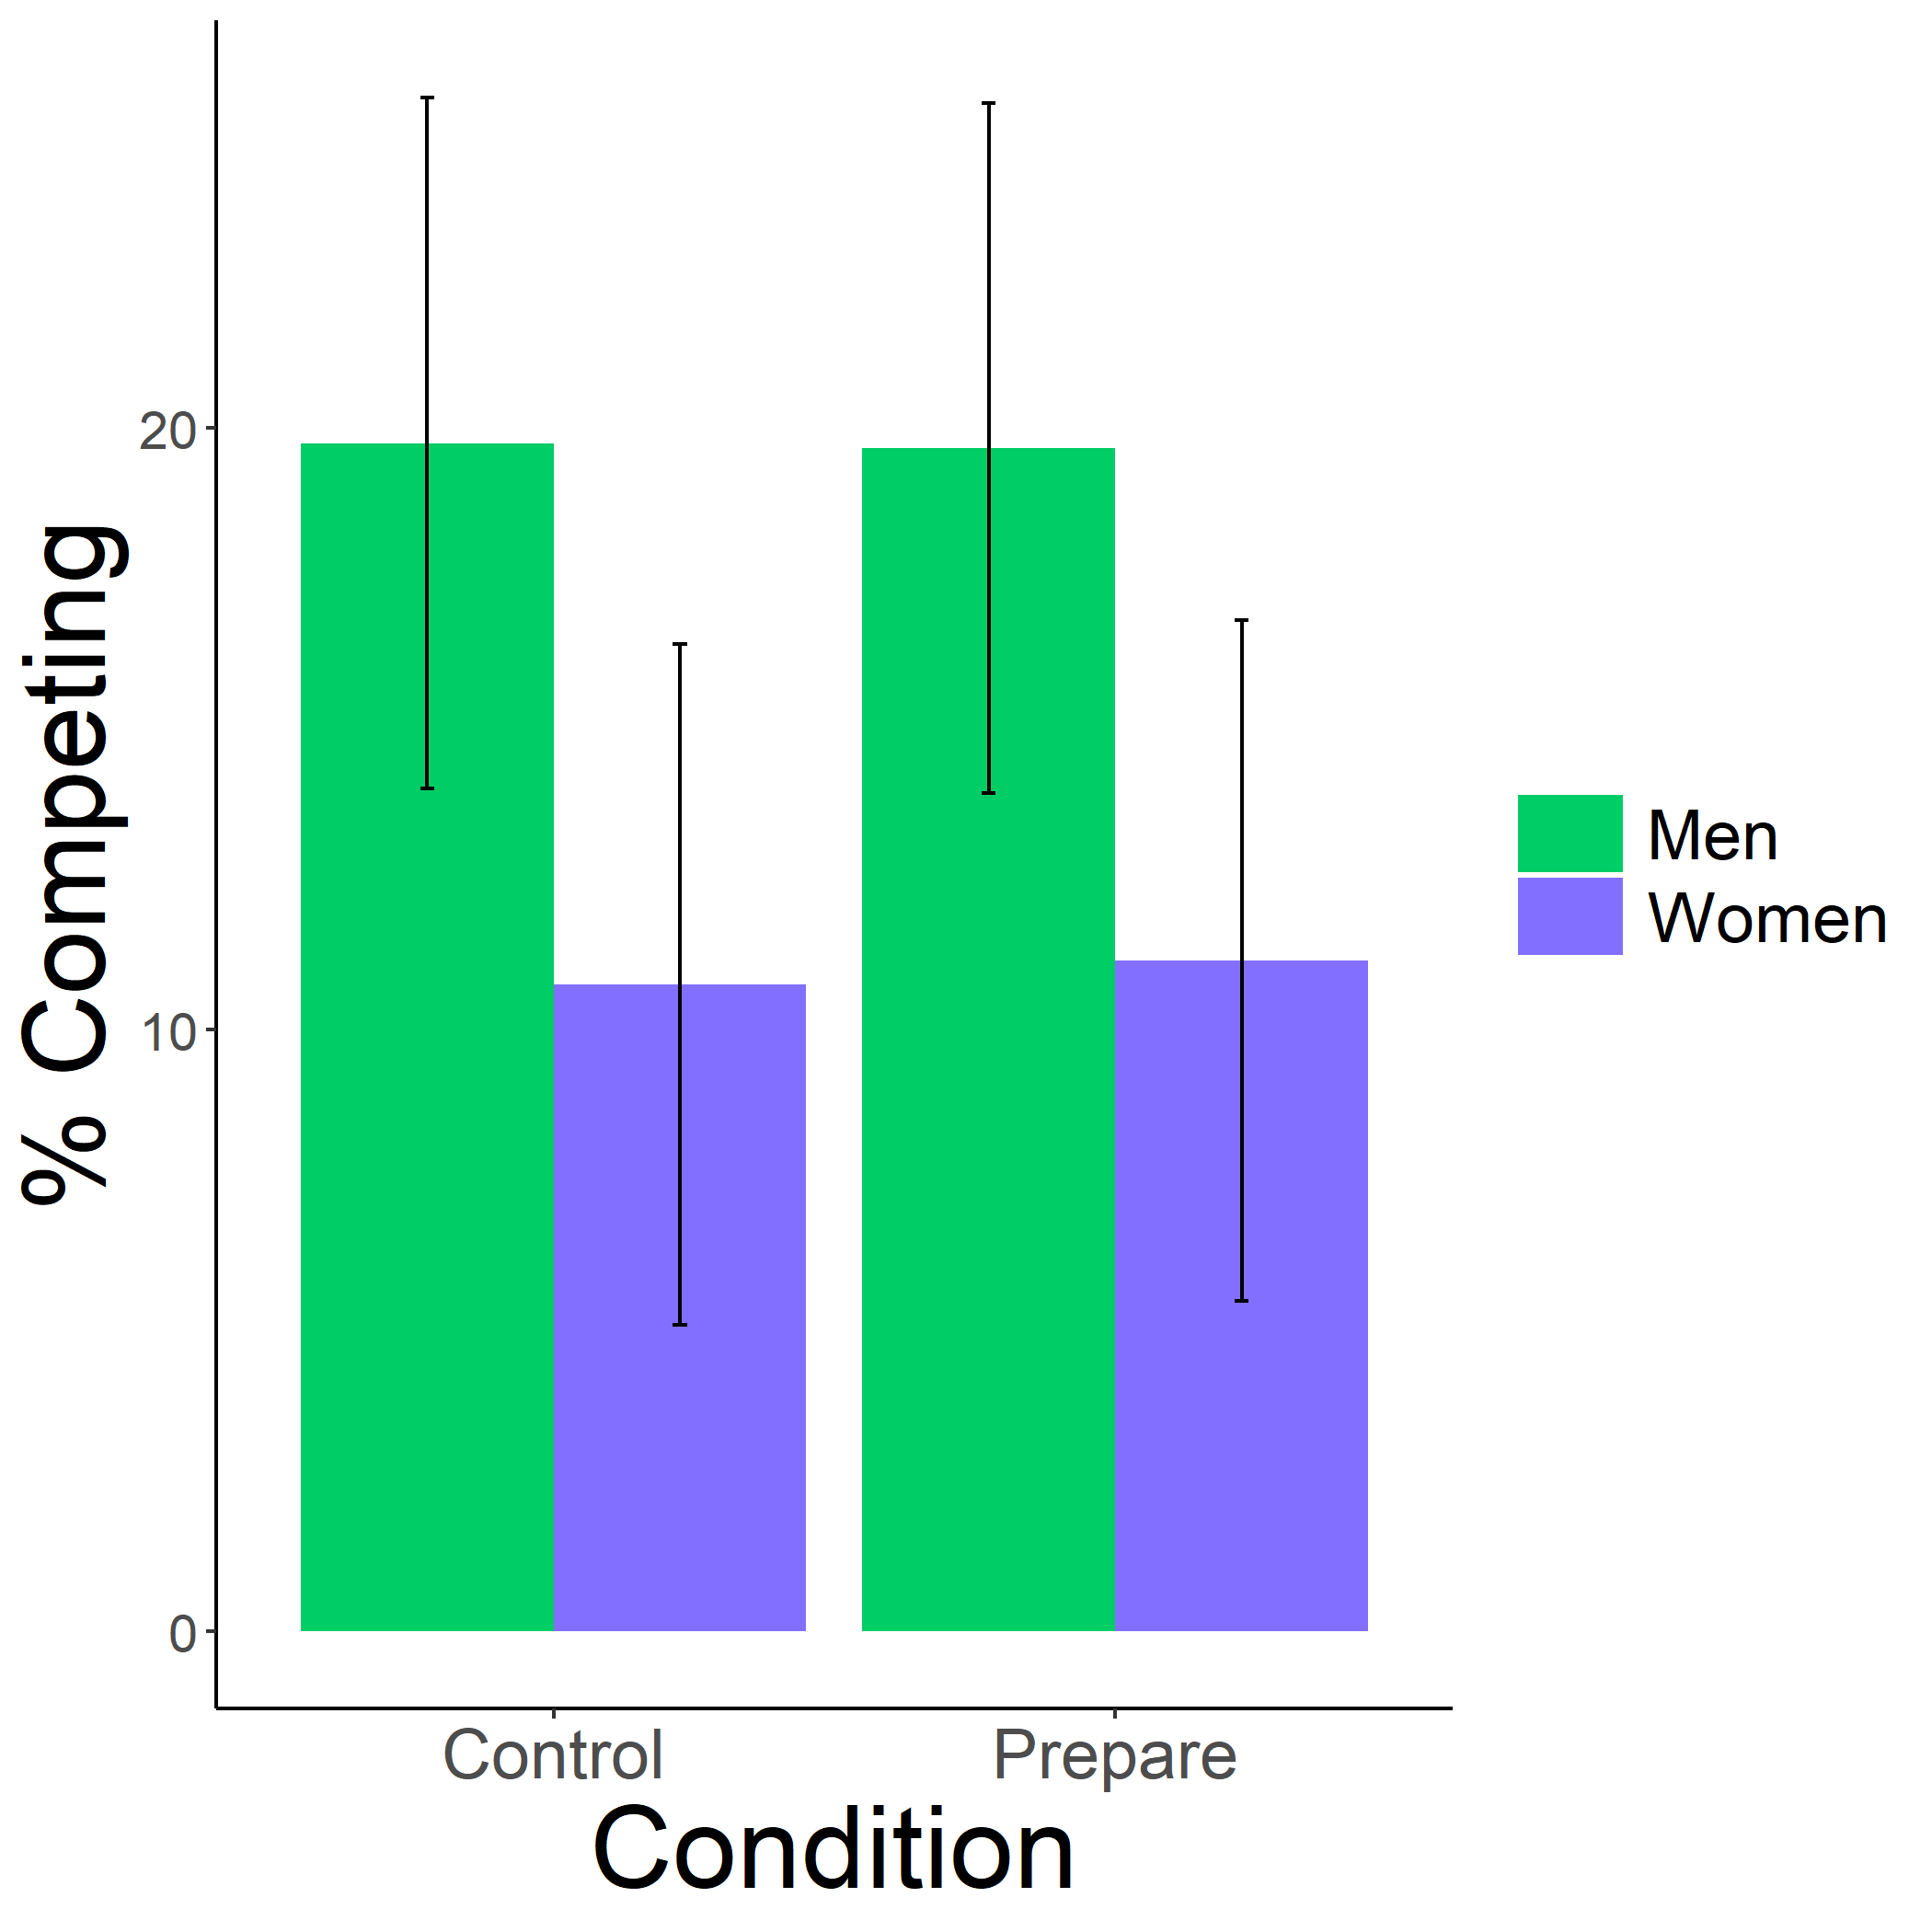
\includegraphics[width=29.17in]{C:/Users/keana/OneDrive - PennO365/Comp_transfer2018/Penn/practice_study/gender-practice/study1/figs/fig00_comp-choice-by-gender-and-cond-bar} \caption{Proportion of male and female participants who chose to compete by condition. We do not find evidence for the hypothesized interaction between gender and condition on the choice to compete, nor do we see a main effect of condition on the choice to compete. Error bars represent standard errors.}\label{fig:s100}
\end{figure}

\begin{figure}
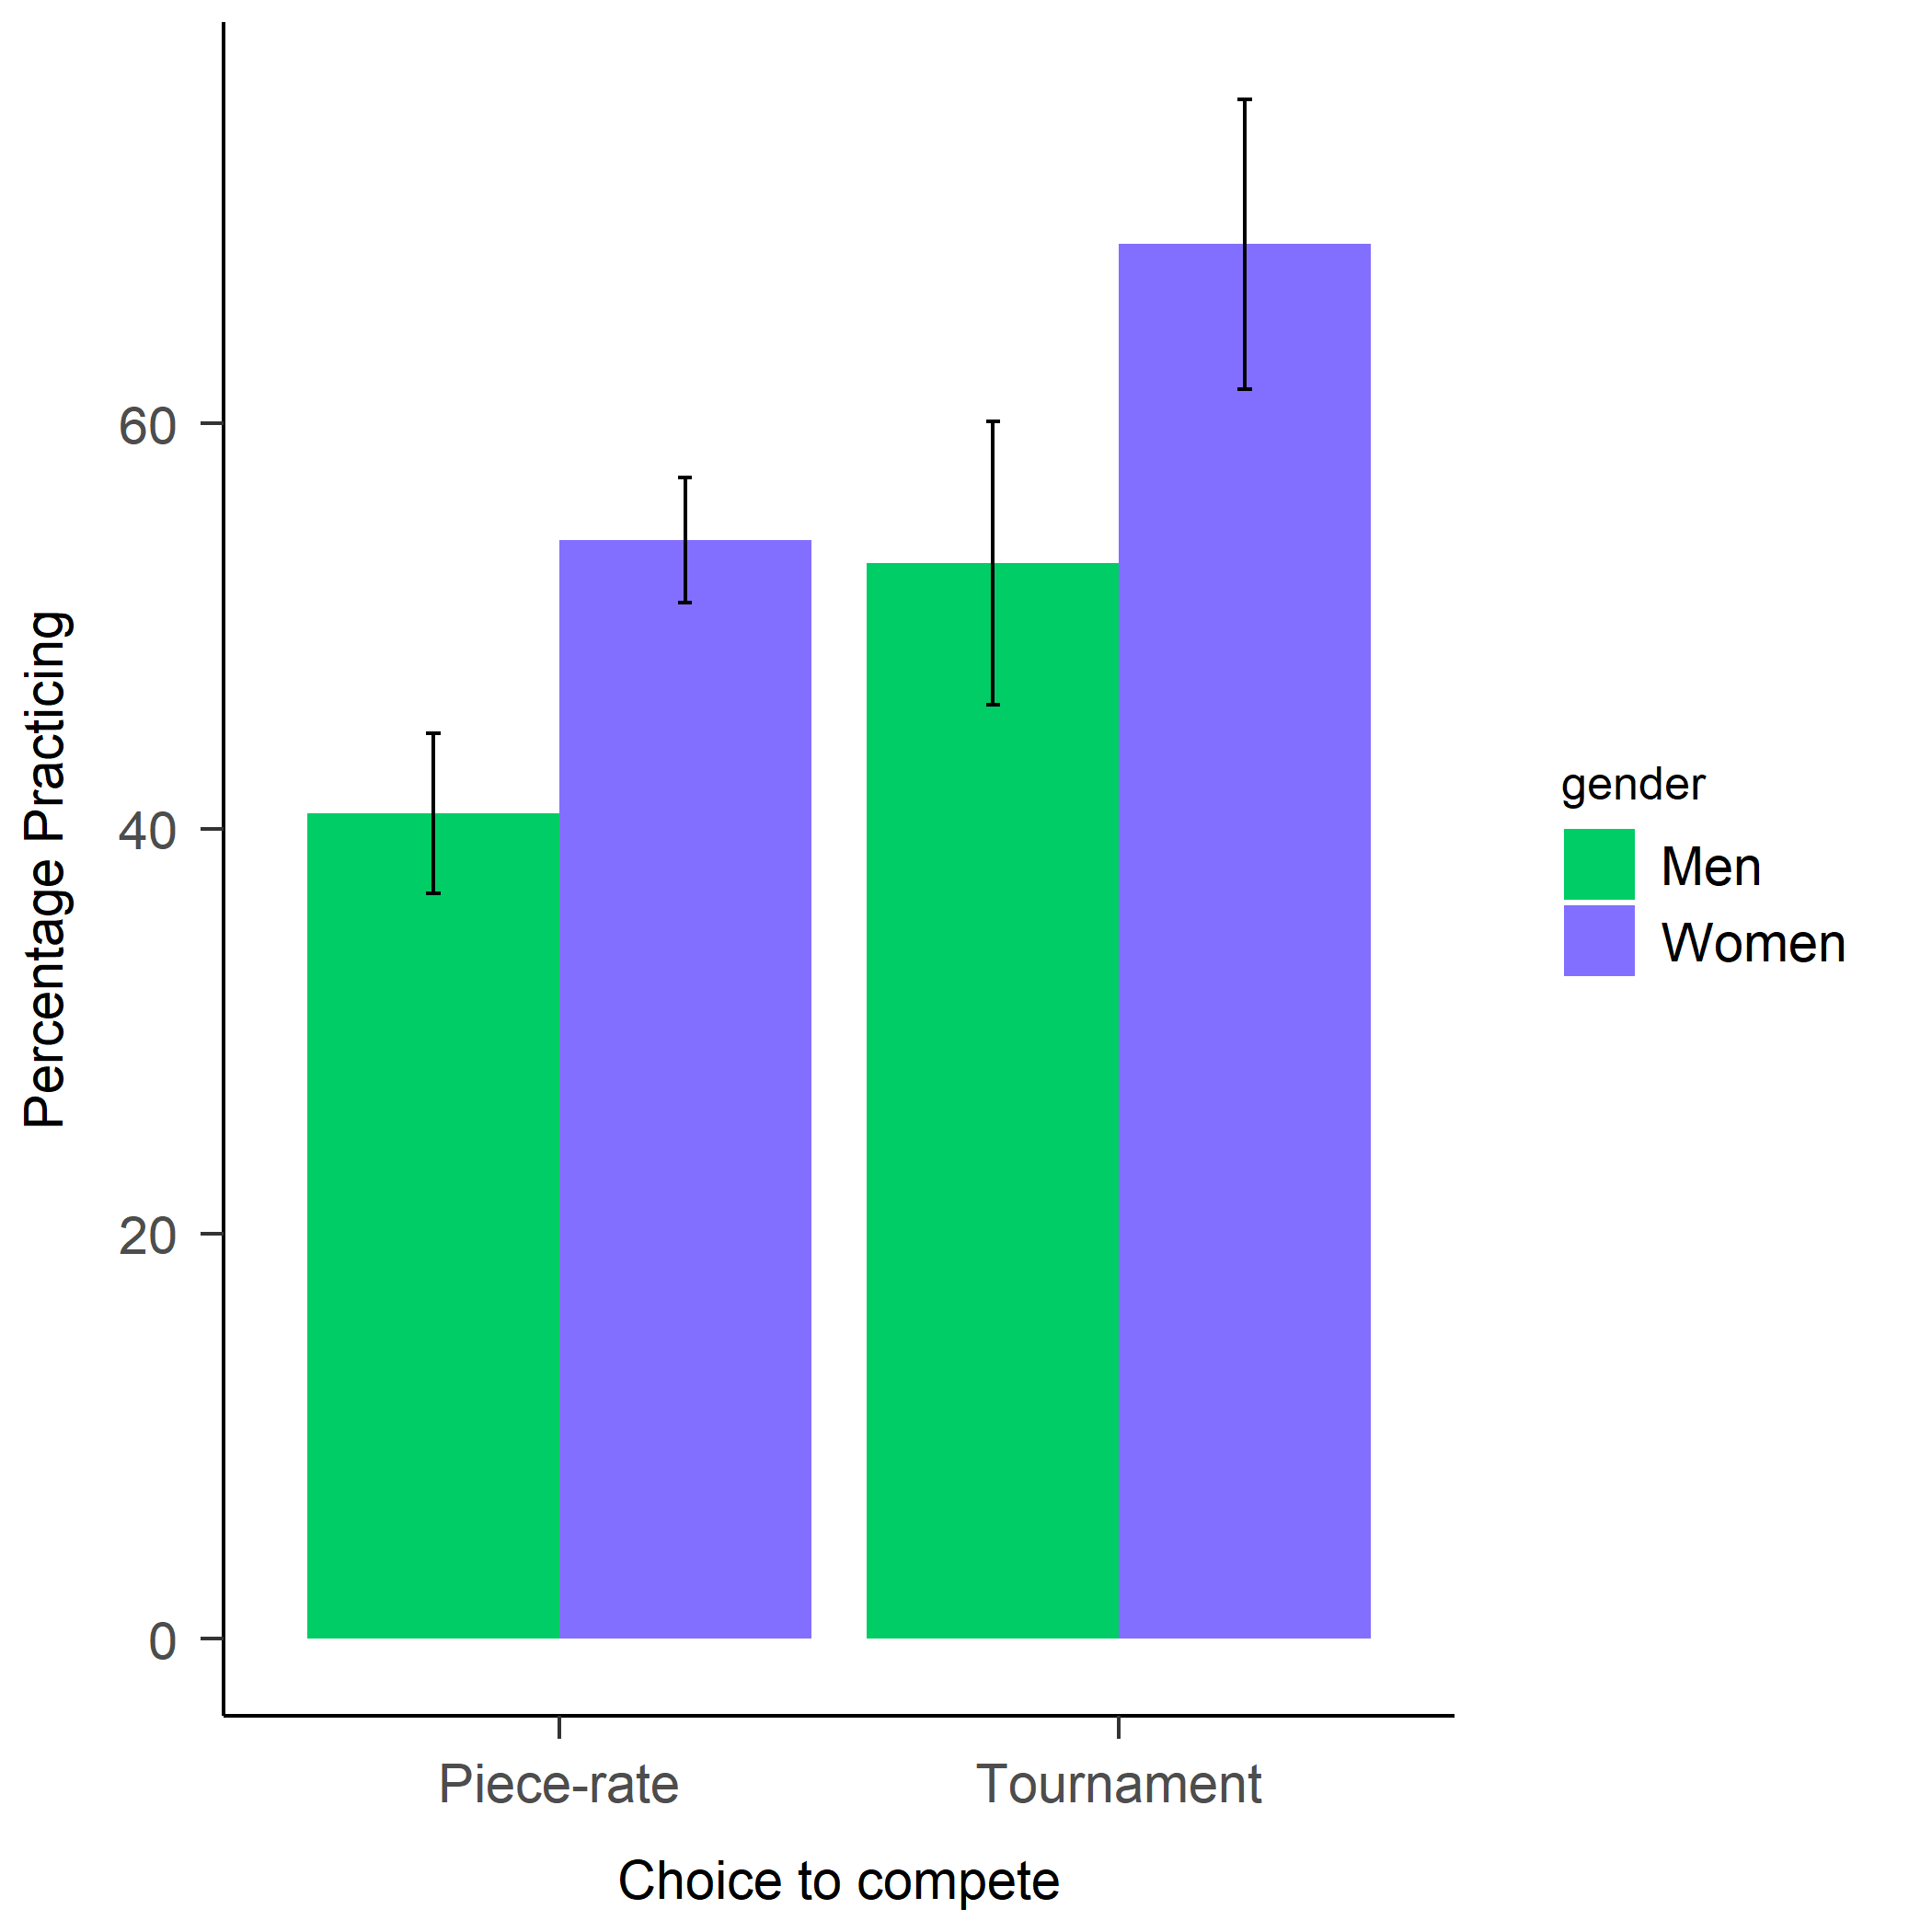
\includegraphics[width=29.17in]{C:/Users/keana/OneDrive - PennO365/Comp_transfer2018/Penn/practice_study/gender-practice/study1/figs/fig01_pract-choice-by-gender-and-comp-choice-bar} \caption{Proportion of male and female participants who chose to prepare by choice to compete. Women are significantly more willing to prepare, even before they know what the preparation involves. There is no interaction between gender and choice to compete on the decision to prepare. Error bars represent standard errors.}\label{fig:s101}
\end{figure}

\begin{figure}
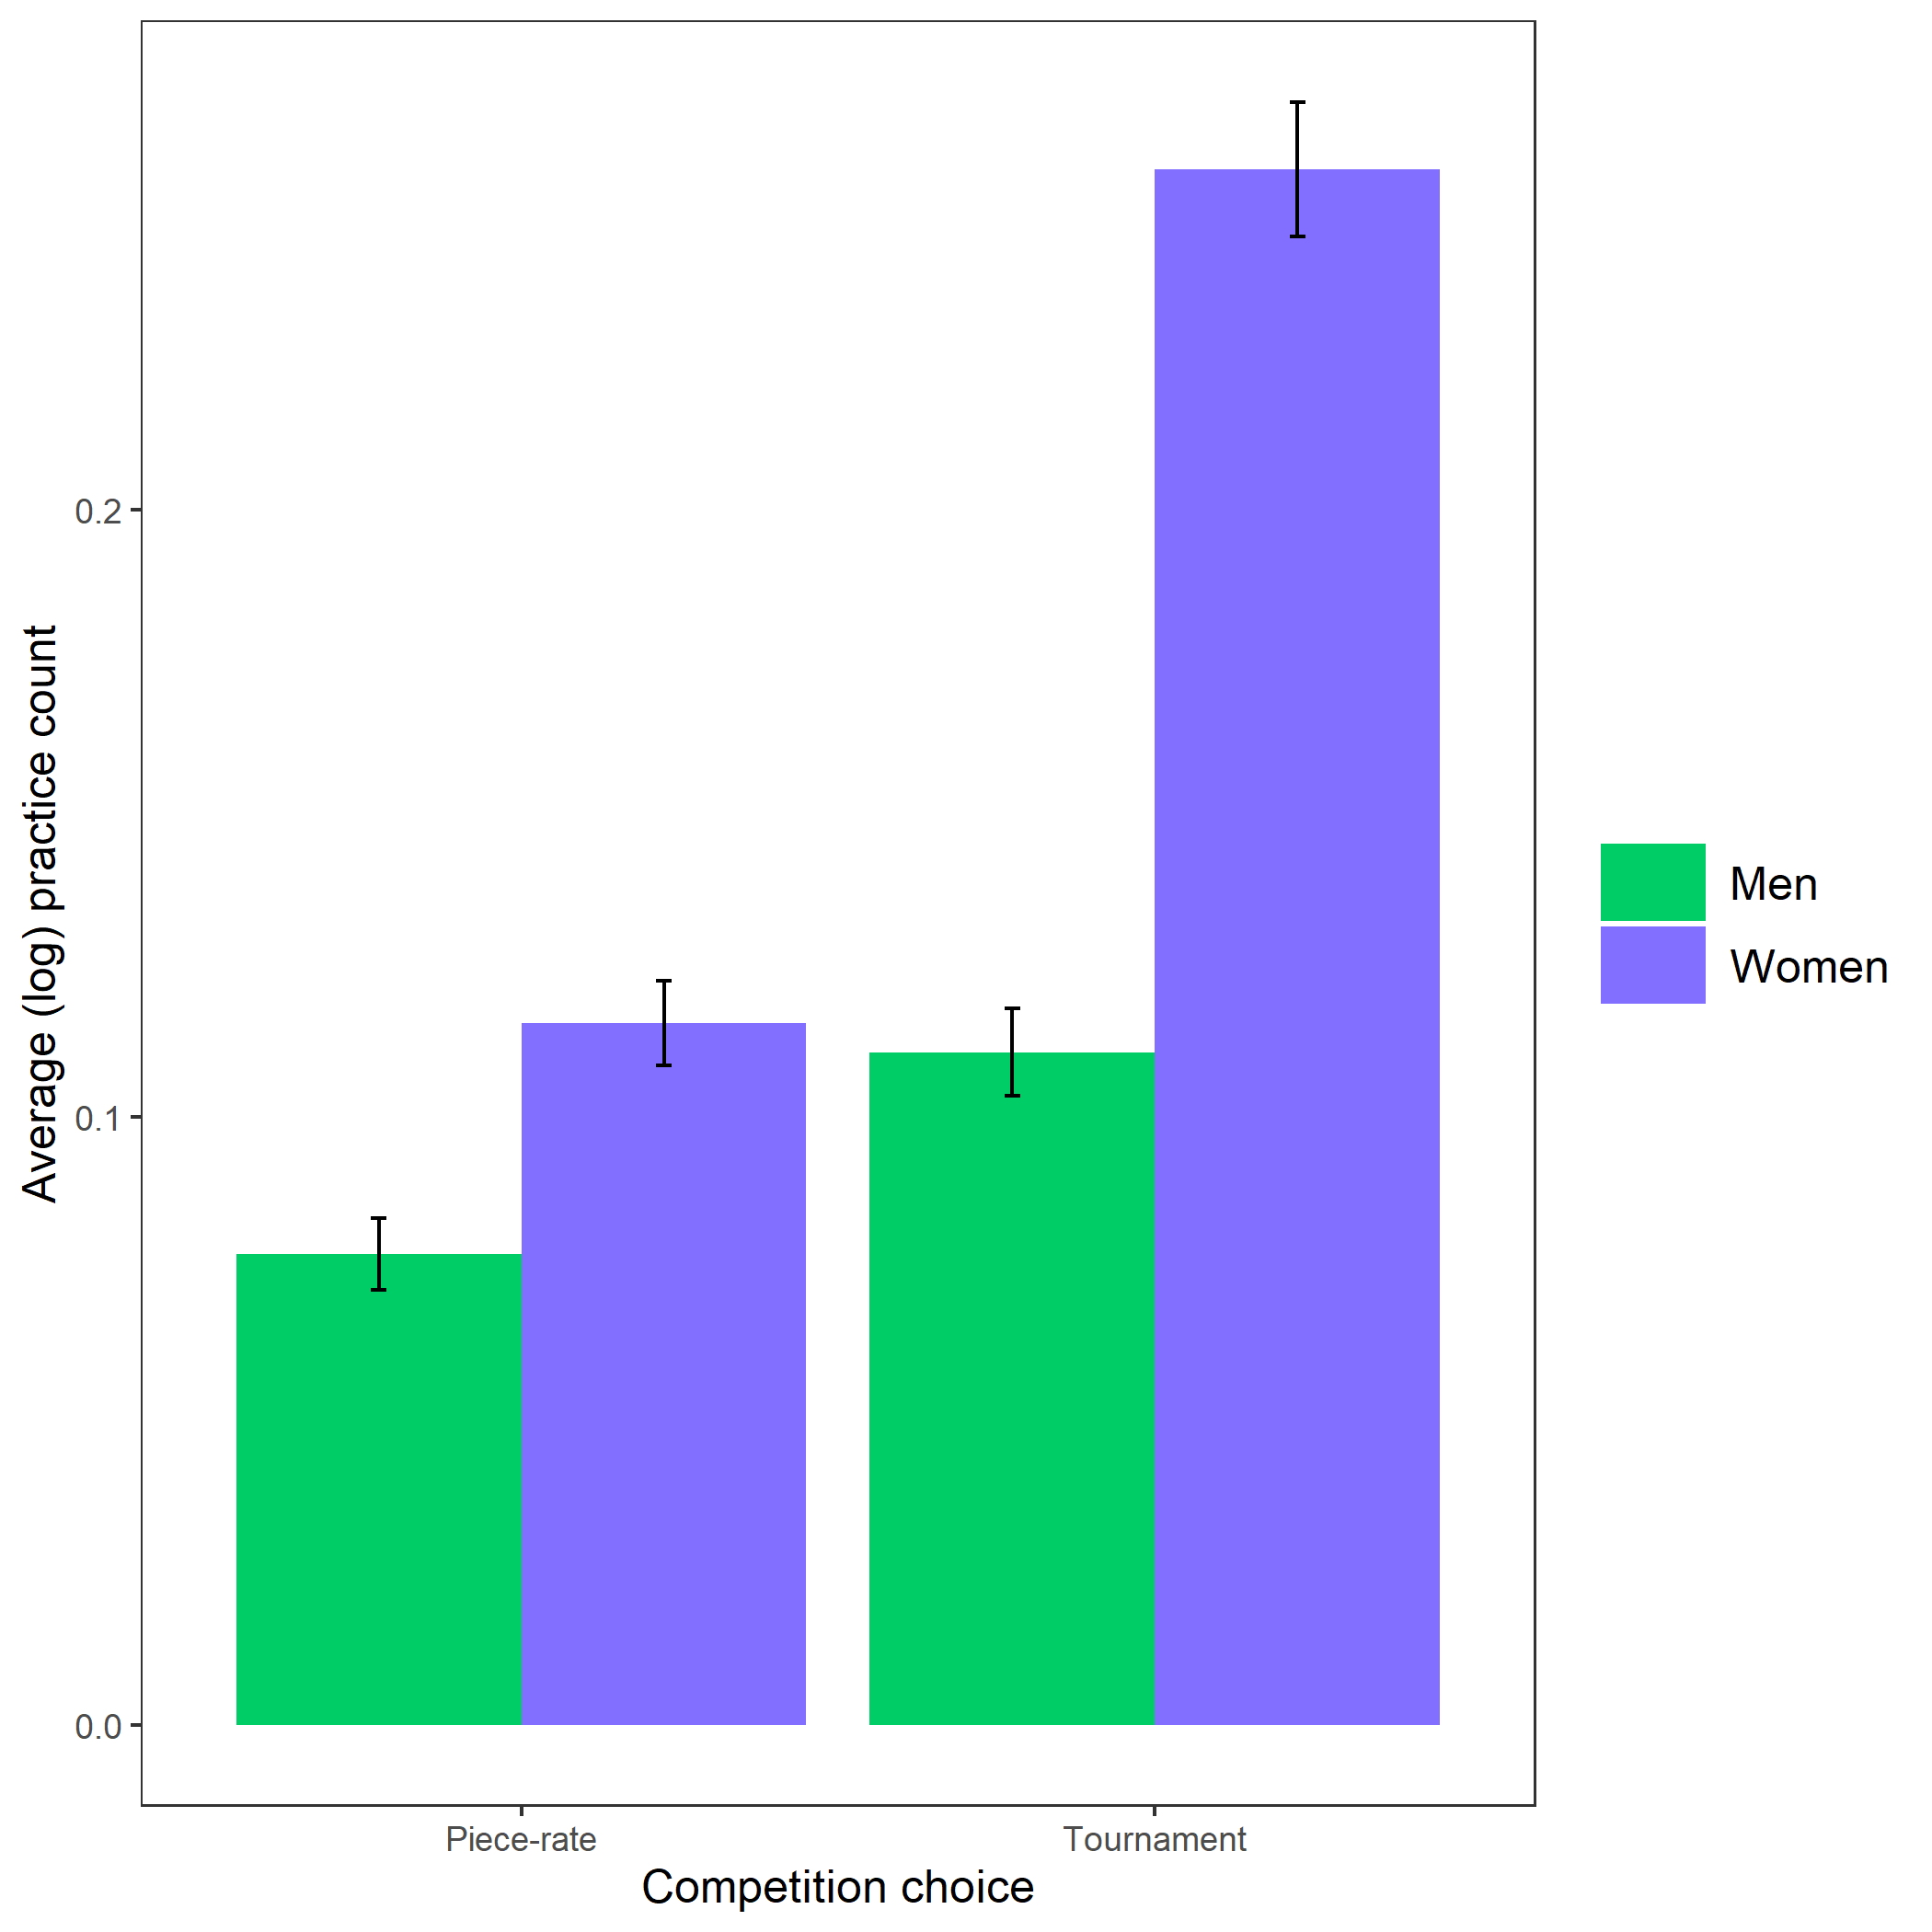
\includegraphics[width=29.17in]{C:/Users/keana/OneDrive - PennO365/Comp_transfer2018/Penn/practice_study/gender-practice/study1/figs/fig02_total-rev-count-by-gender-comp-choice} \caption{Average (log-transformed) practice count based on participant gender and competition choice. We find further evidence of a gender difference in the choice to prepare using a different metric of the choice to prepare: the number of times a participant chooses to persist in their practice effort by repeatedly practicing. Here, we find evidence of a significant interaction between gender and the choice to compete on the choice to practice, where women who chose to compete are significantly more likely to practice. However, the small size of this cell must be considered when interpreting this interaction. Future research is needed to ensure this effect replicates. Error bars represent standard errors.}\label{fig:s102}
\end{figure}

\begin{figure}
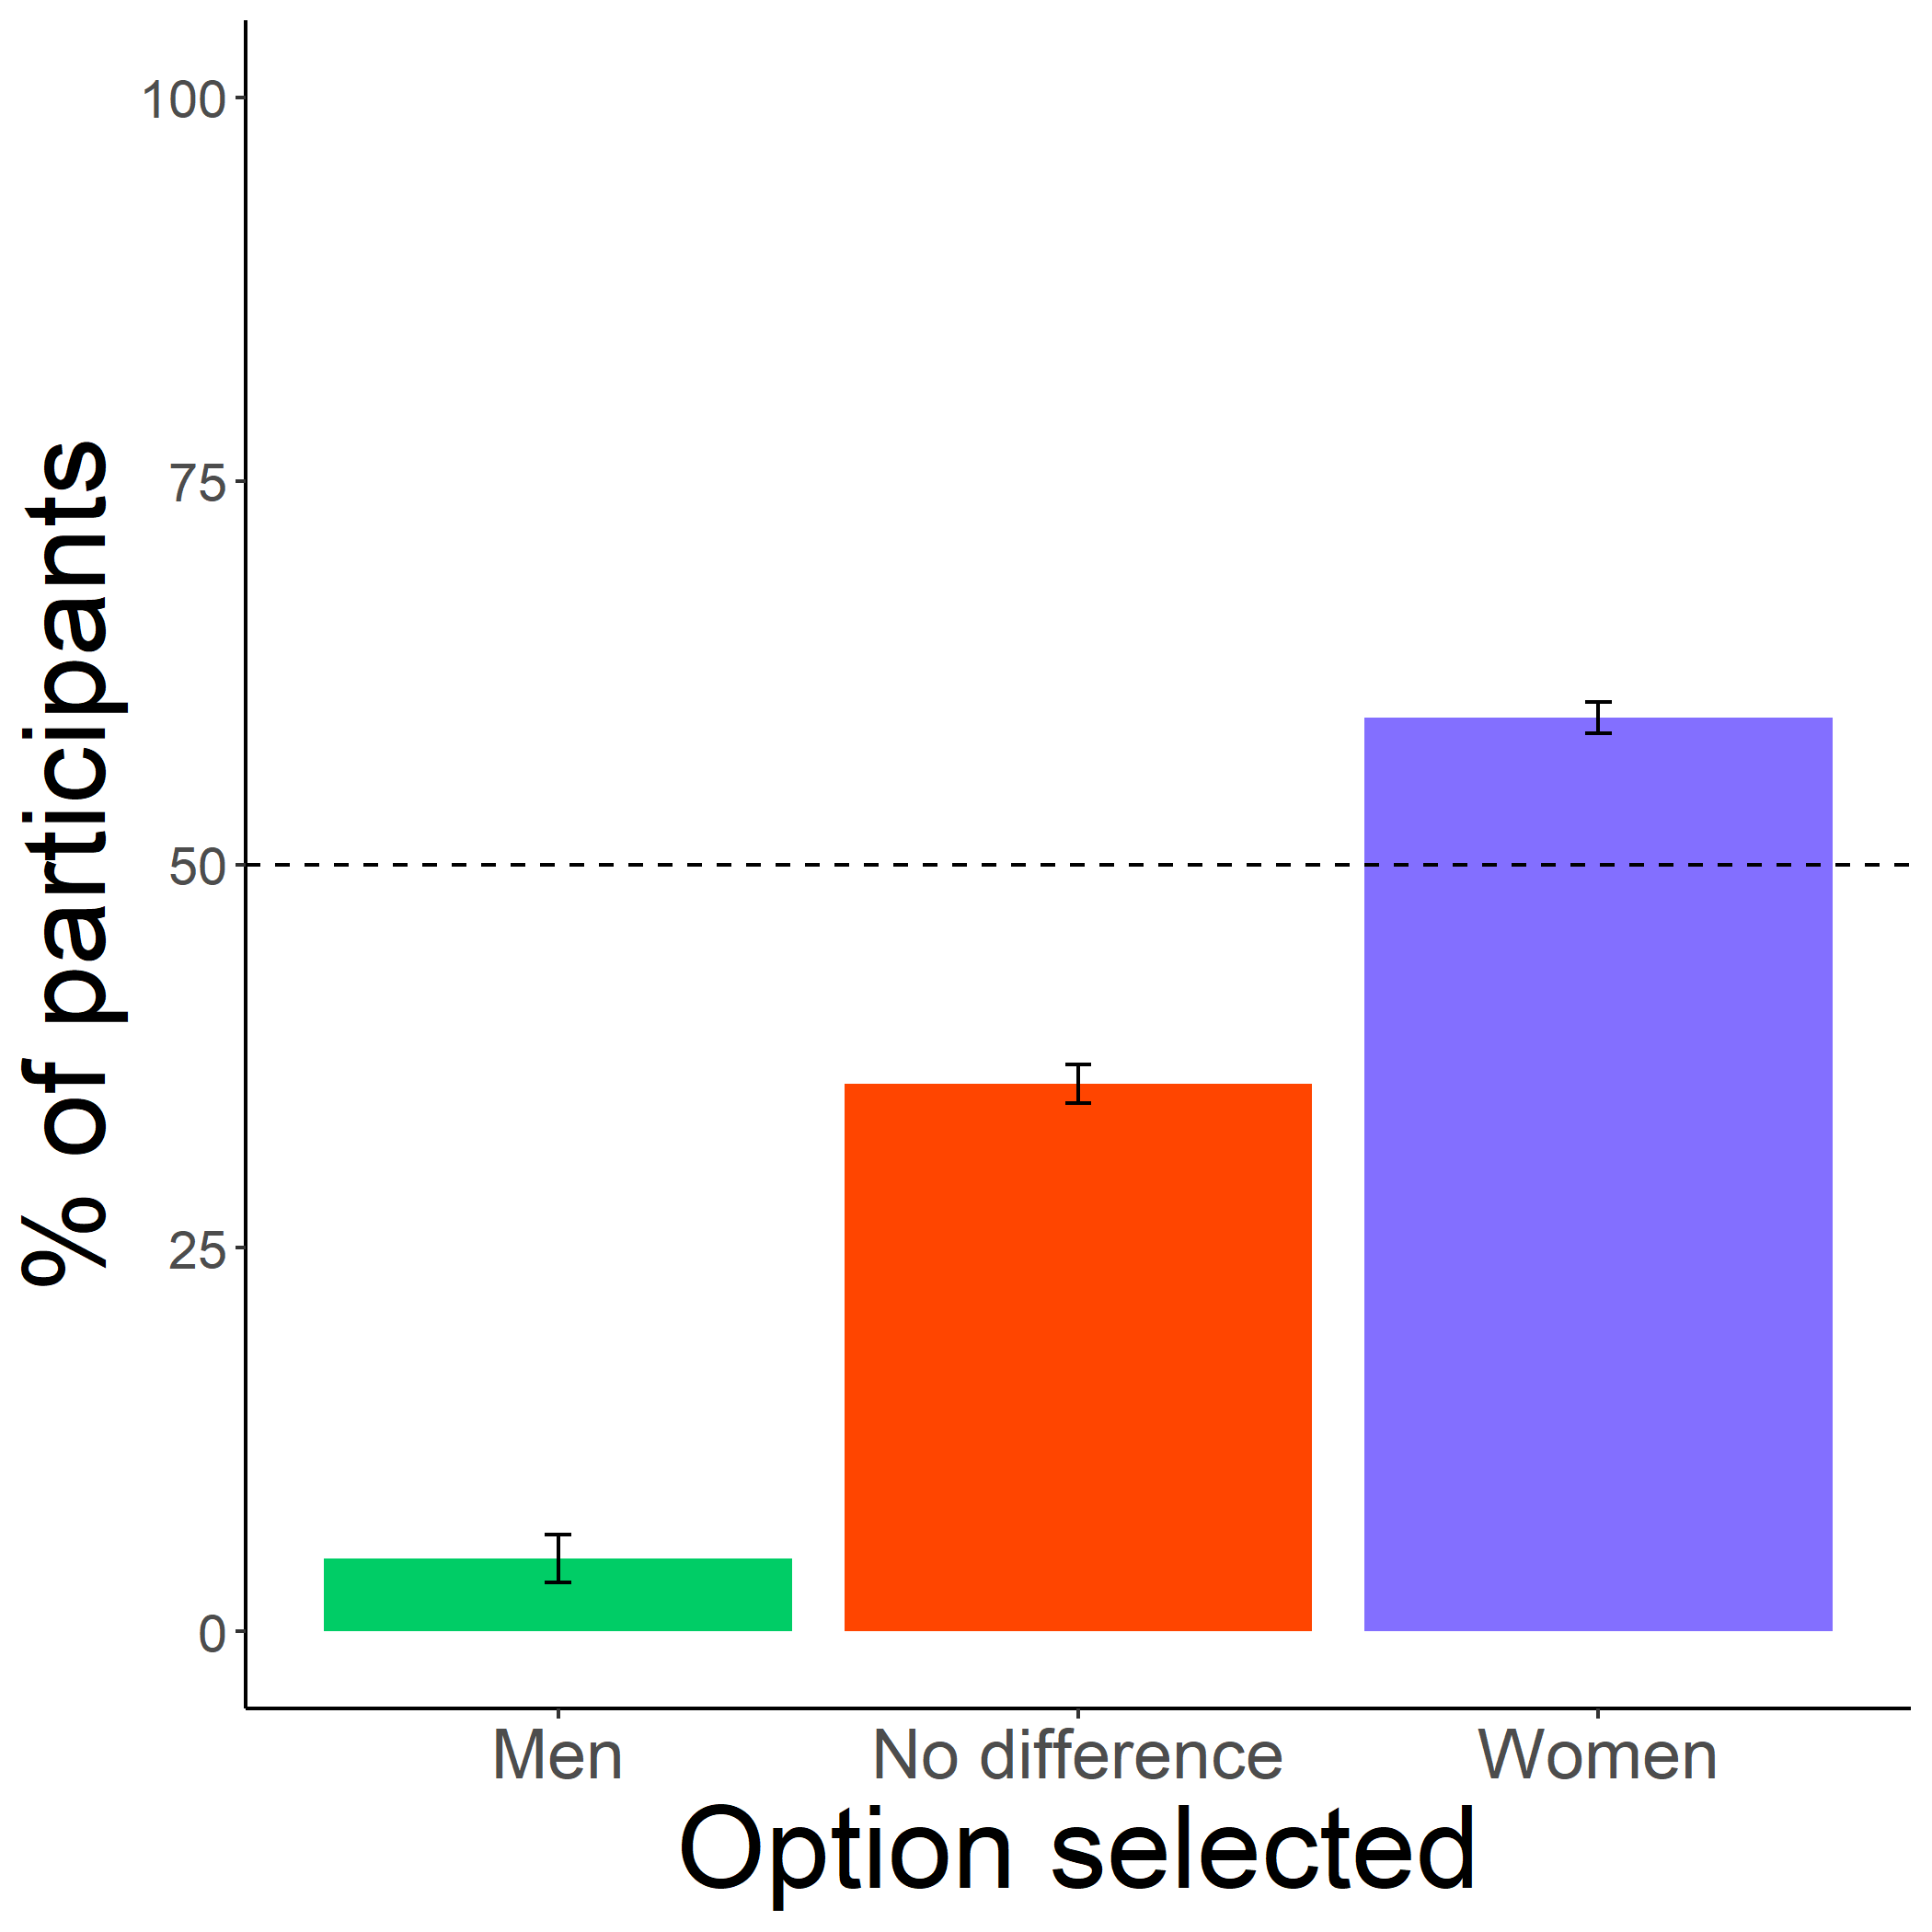
\includegraphics[width=29.17in]{C:/Users/keana/OneDrive - PennO365/Comp_transfer2018/Penn/practice_study/gender-practice/study1/figs/fig03_perc-task-gender-pract} \caption{Participants' perceptions of gender differences in the choice to practice on the task. Both men and women correctly anticipate that women will be more willing to practice before completing the multiplication task. Women are especially likely to state women will prepare more for the task. Error bars represent standard errors.}\label{fig:s103}
\end{figure}

\begin{figure}
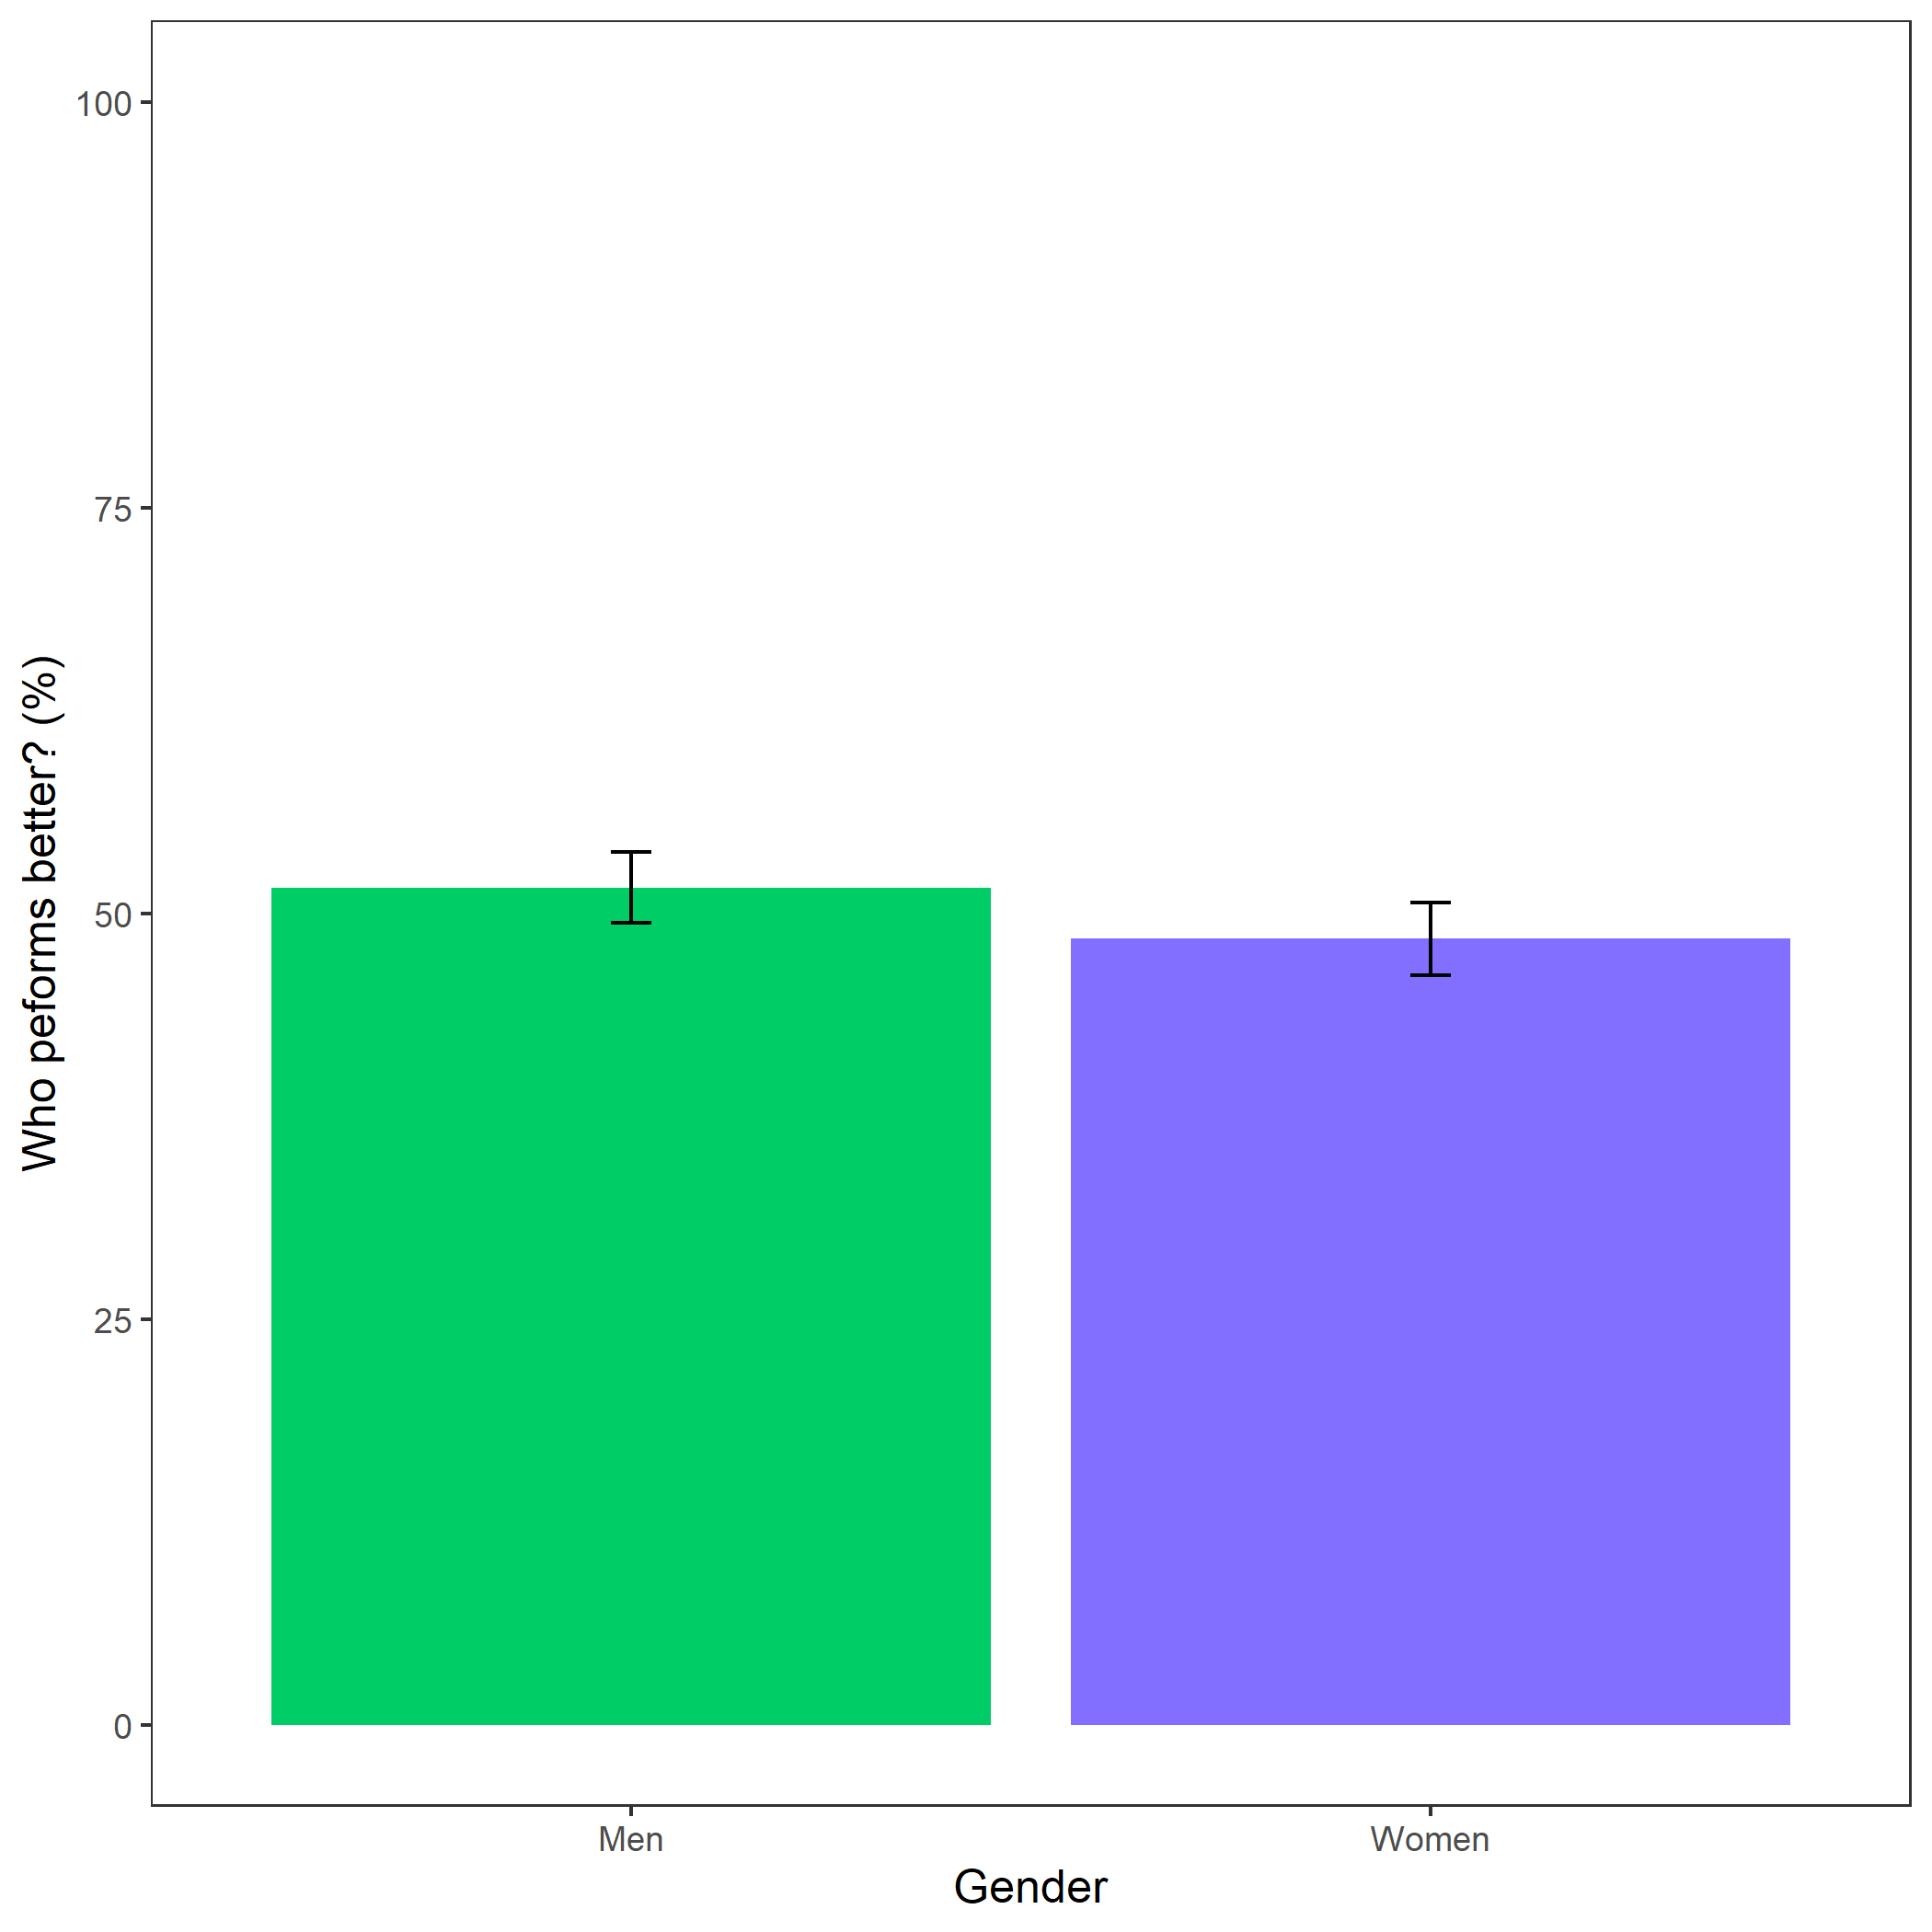
\includegraphics[width=29.17in]{C:/Users/keana/OneDrive - PennO365/Comp_transfer2018/Penn/practice_study/gender-practice/study1/figs/fig04_better-gender-guess} \caption{Participants' perceptions of gender differences in performance on the task. Participants were equally likely to predict that women (vs. men) would perform better on the task, suggesting that participants did not have strong stereotypes about gender differences in performance on the multiplication task. Error bars represent standard errors.}\label{fig:s104}
\end{figure}

\begin{figure}
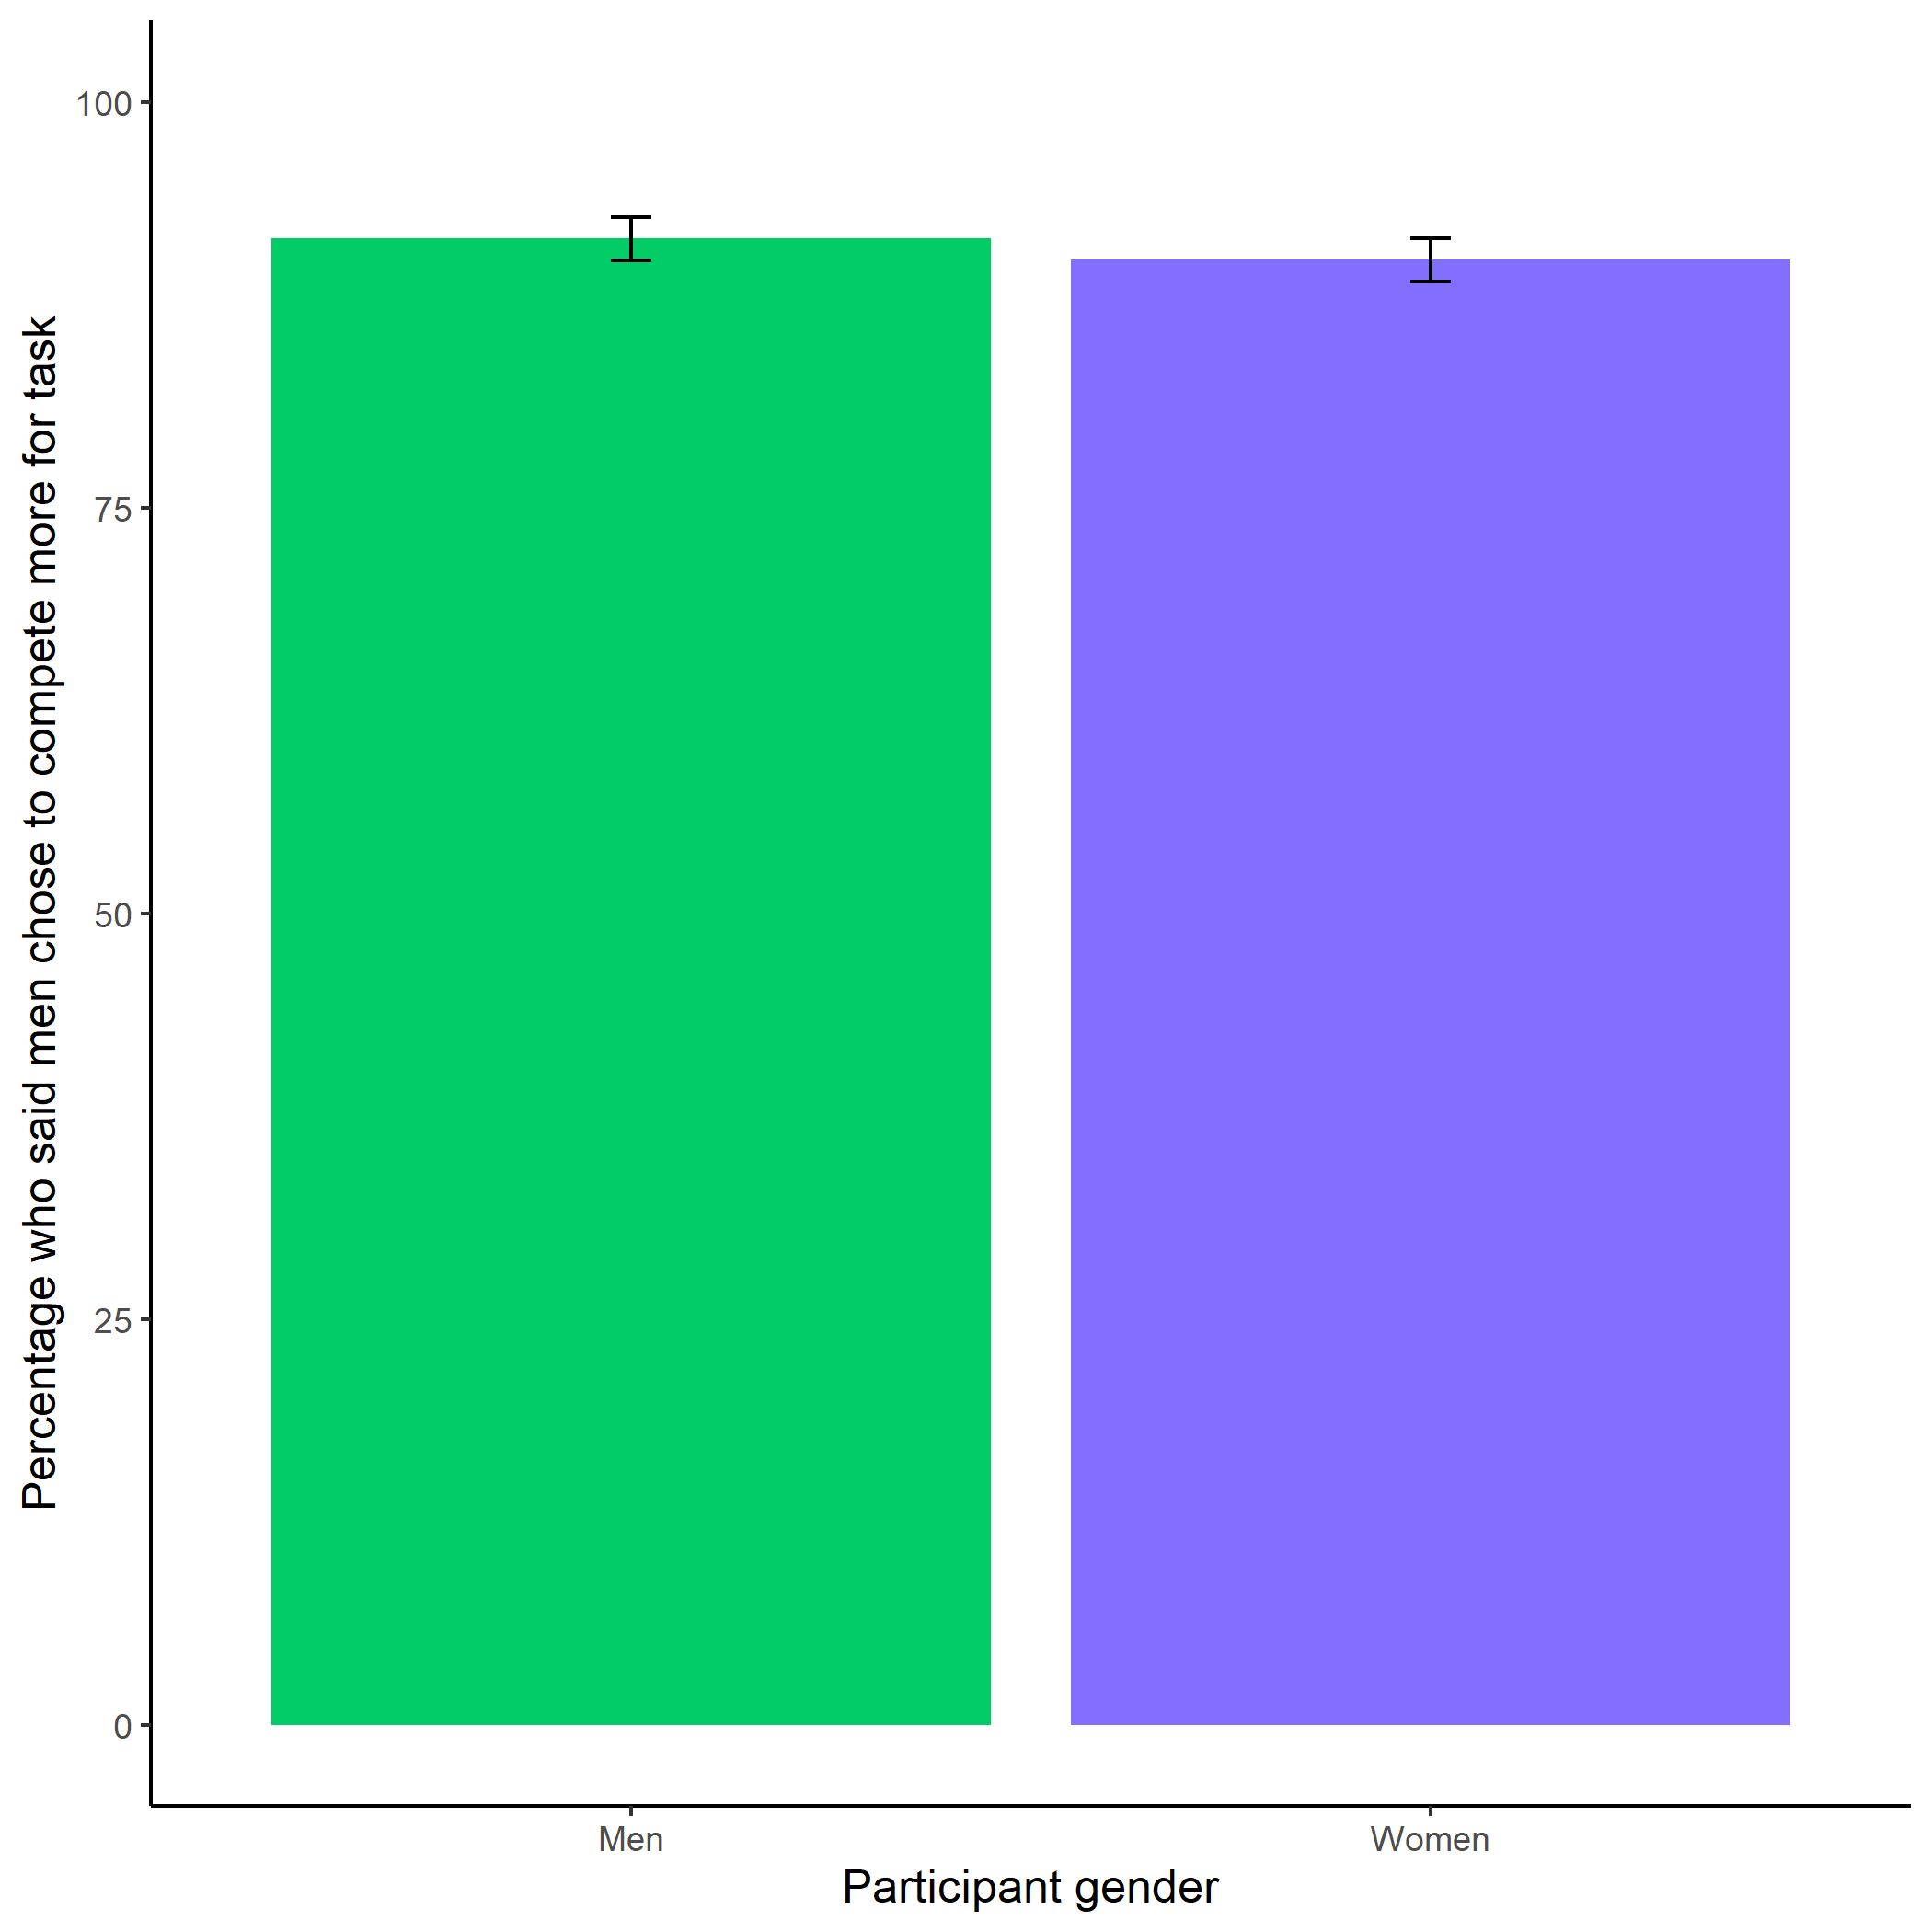
\includegraphics[width=29.17in]{C:/Users/keana/OneDrive - PennO365/Comp_transfer2018/Penn/practice_study/gender-practice/study1/figs/fig05_perc-gender-comp} \caption{Participants' perceptions of gender differences in choice to compete. Both men and women were significantly more likely than chance to correctly state that men would be more likely to choose to compete during the multiplication task, suggesting strong stereotypes about gender differences in competitiveness. Error bars represent standard errors.}\label{fig:s105}
\end{figure}

\begin{figure}
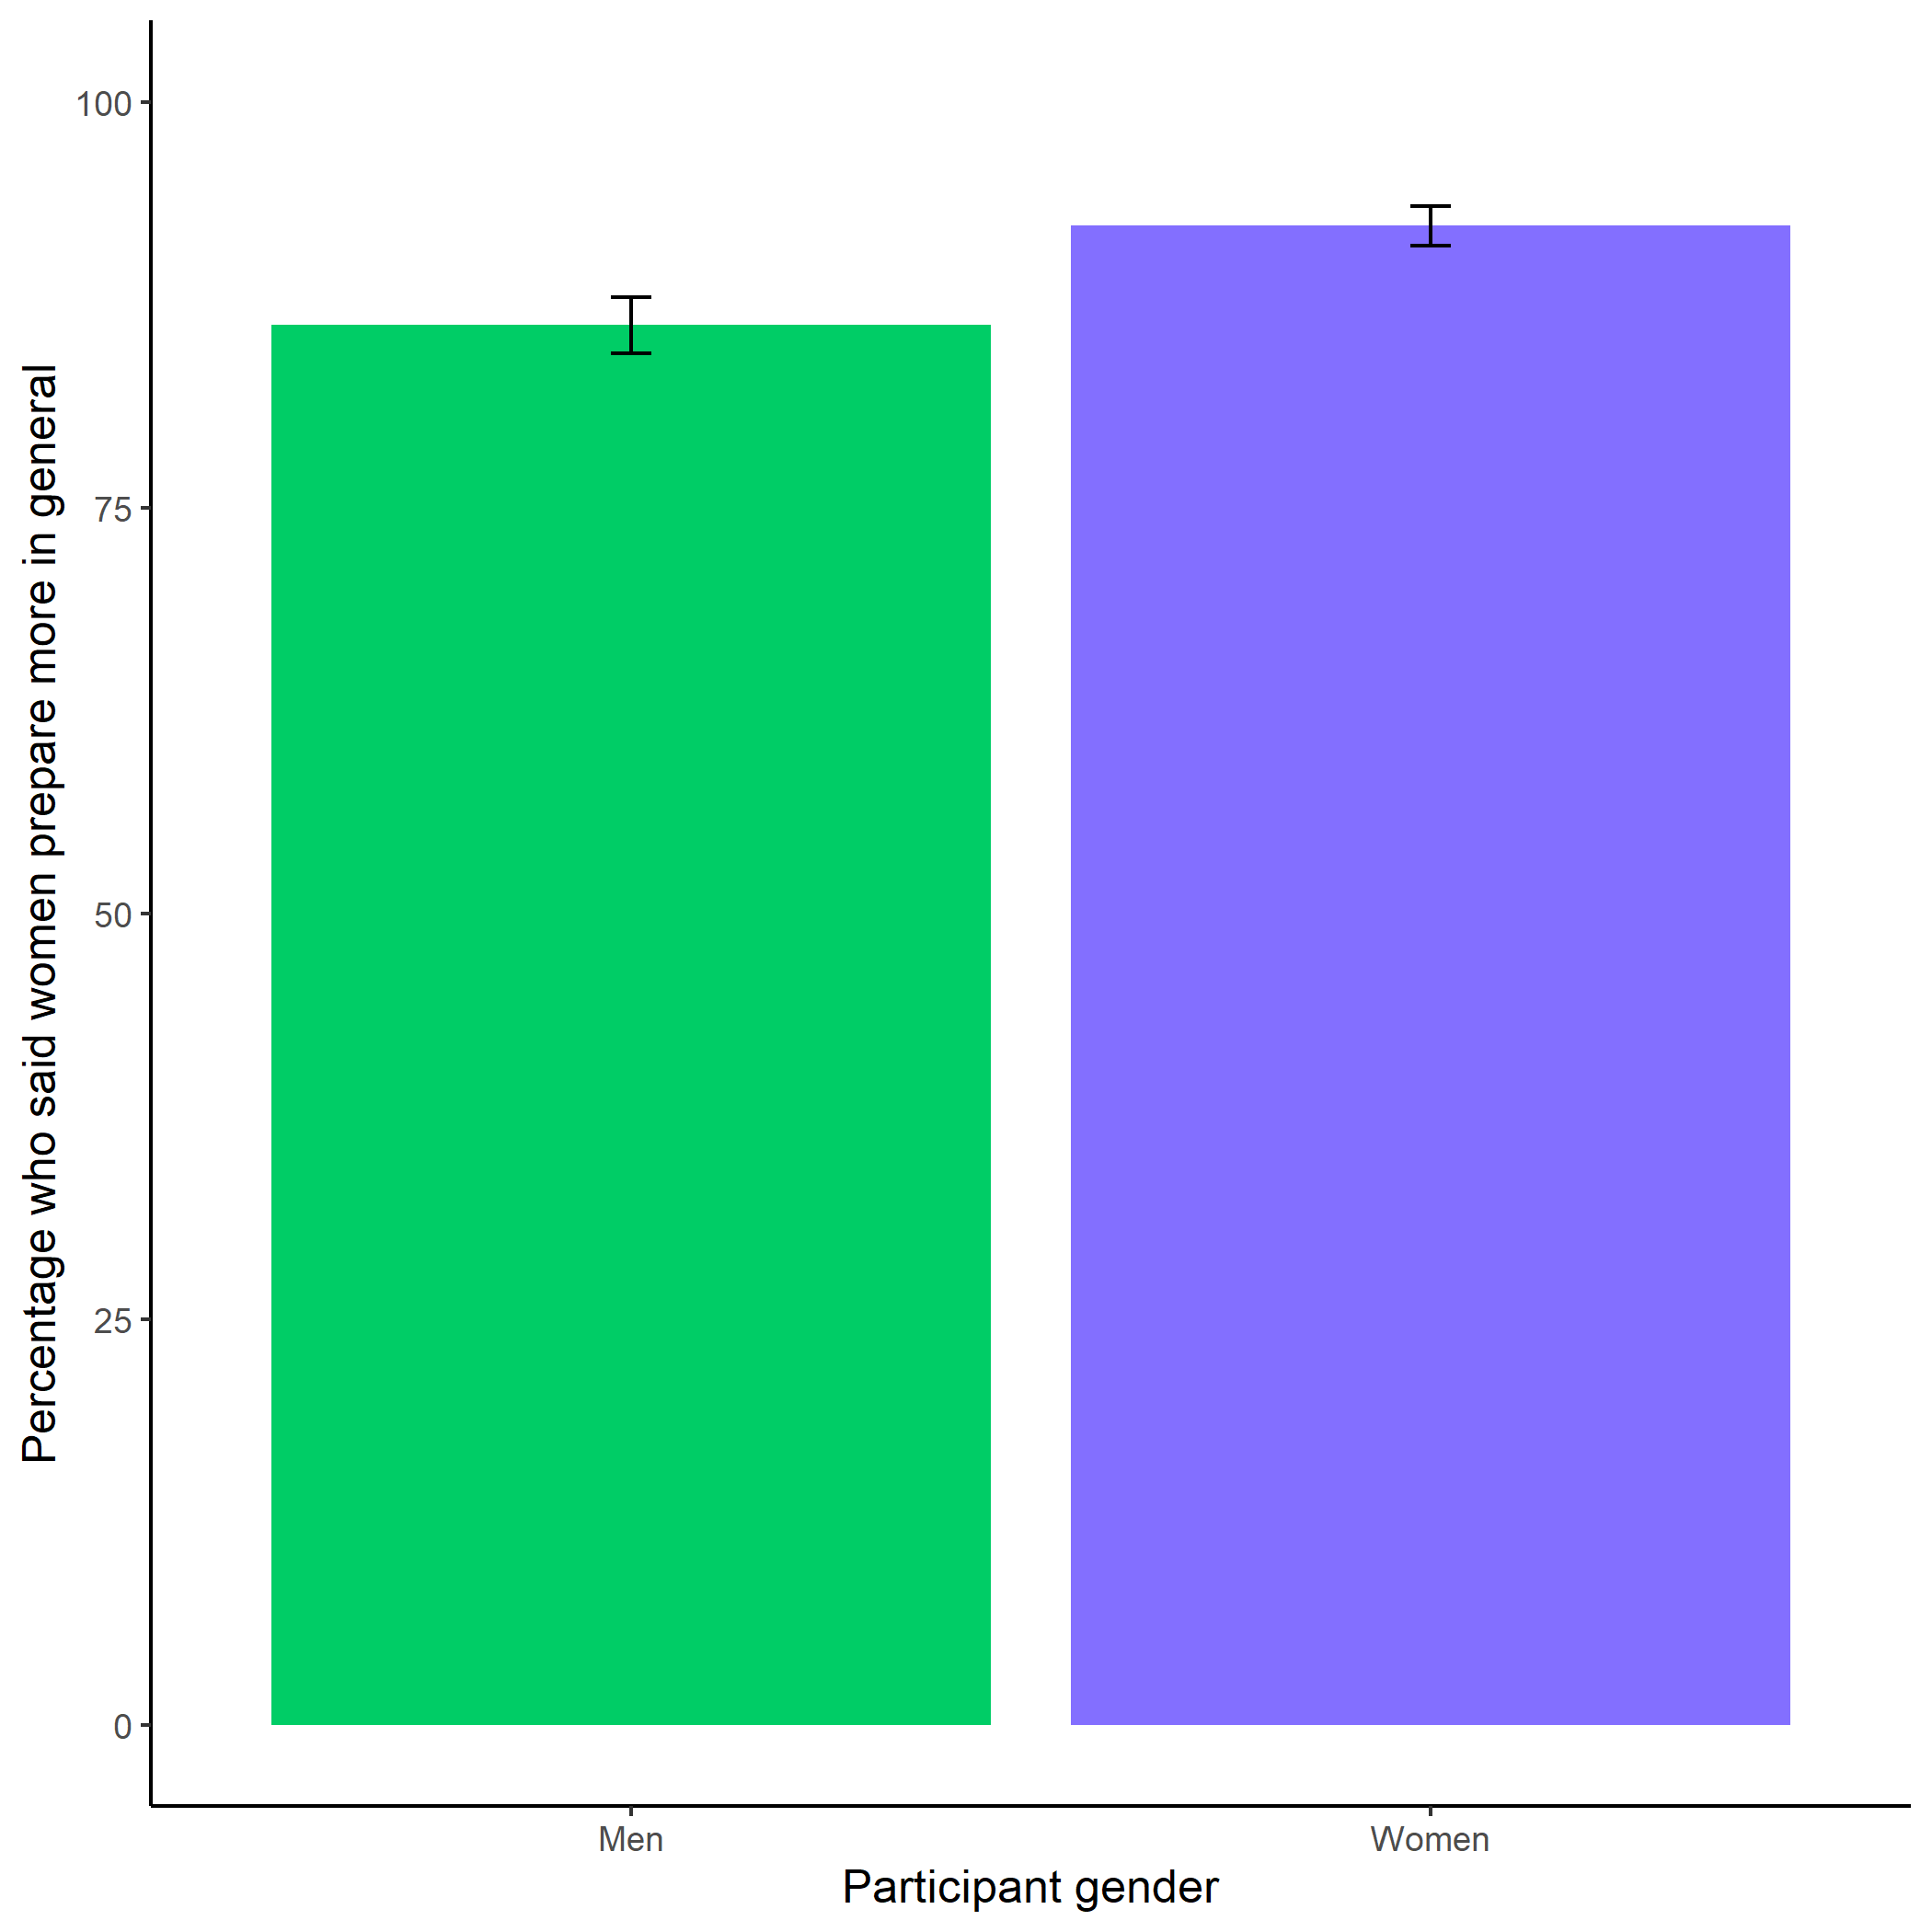
\includegraphics[width=29.17in]{C:/Users/keana/OneDrive - PennO365/Comp_transfer2018/Penn/practice_study/gender-practice/study1/figs/fig06_perc-gen-gender-pract} \caption{Participants' perceptions of general gender differences in choice to practice. Both men and women (but especially women) were significantly more likely than chance to say that women prepare more in general than men. Again, these findings suggest that participants observe these gender differences directly or are aware of stereotypes about gender differences in the choice to prepare. Error bars represent standard errors.}\label{fig:s106}
\end{figure}

\hypertarget{study-2-1}{%
\section{Study 2}\label{study-2-1}}

\begin{figure}
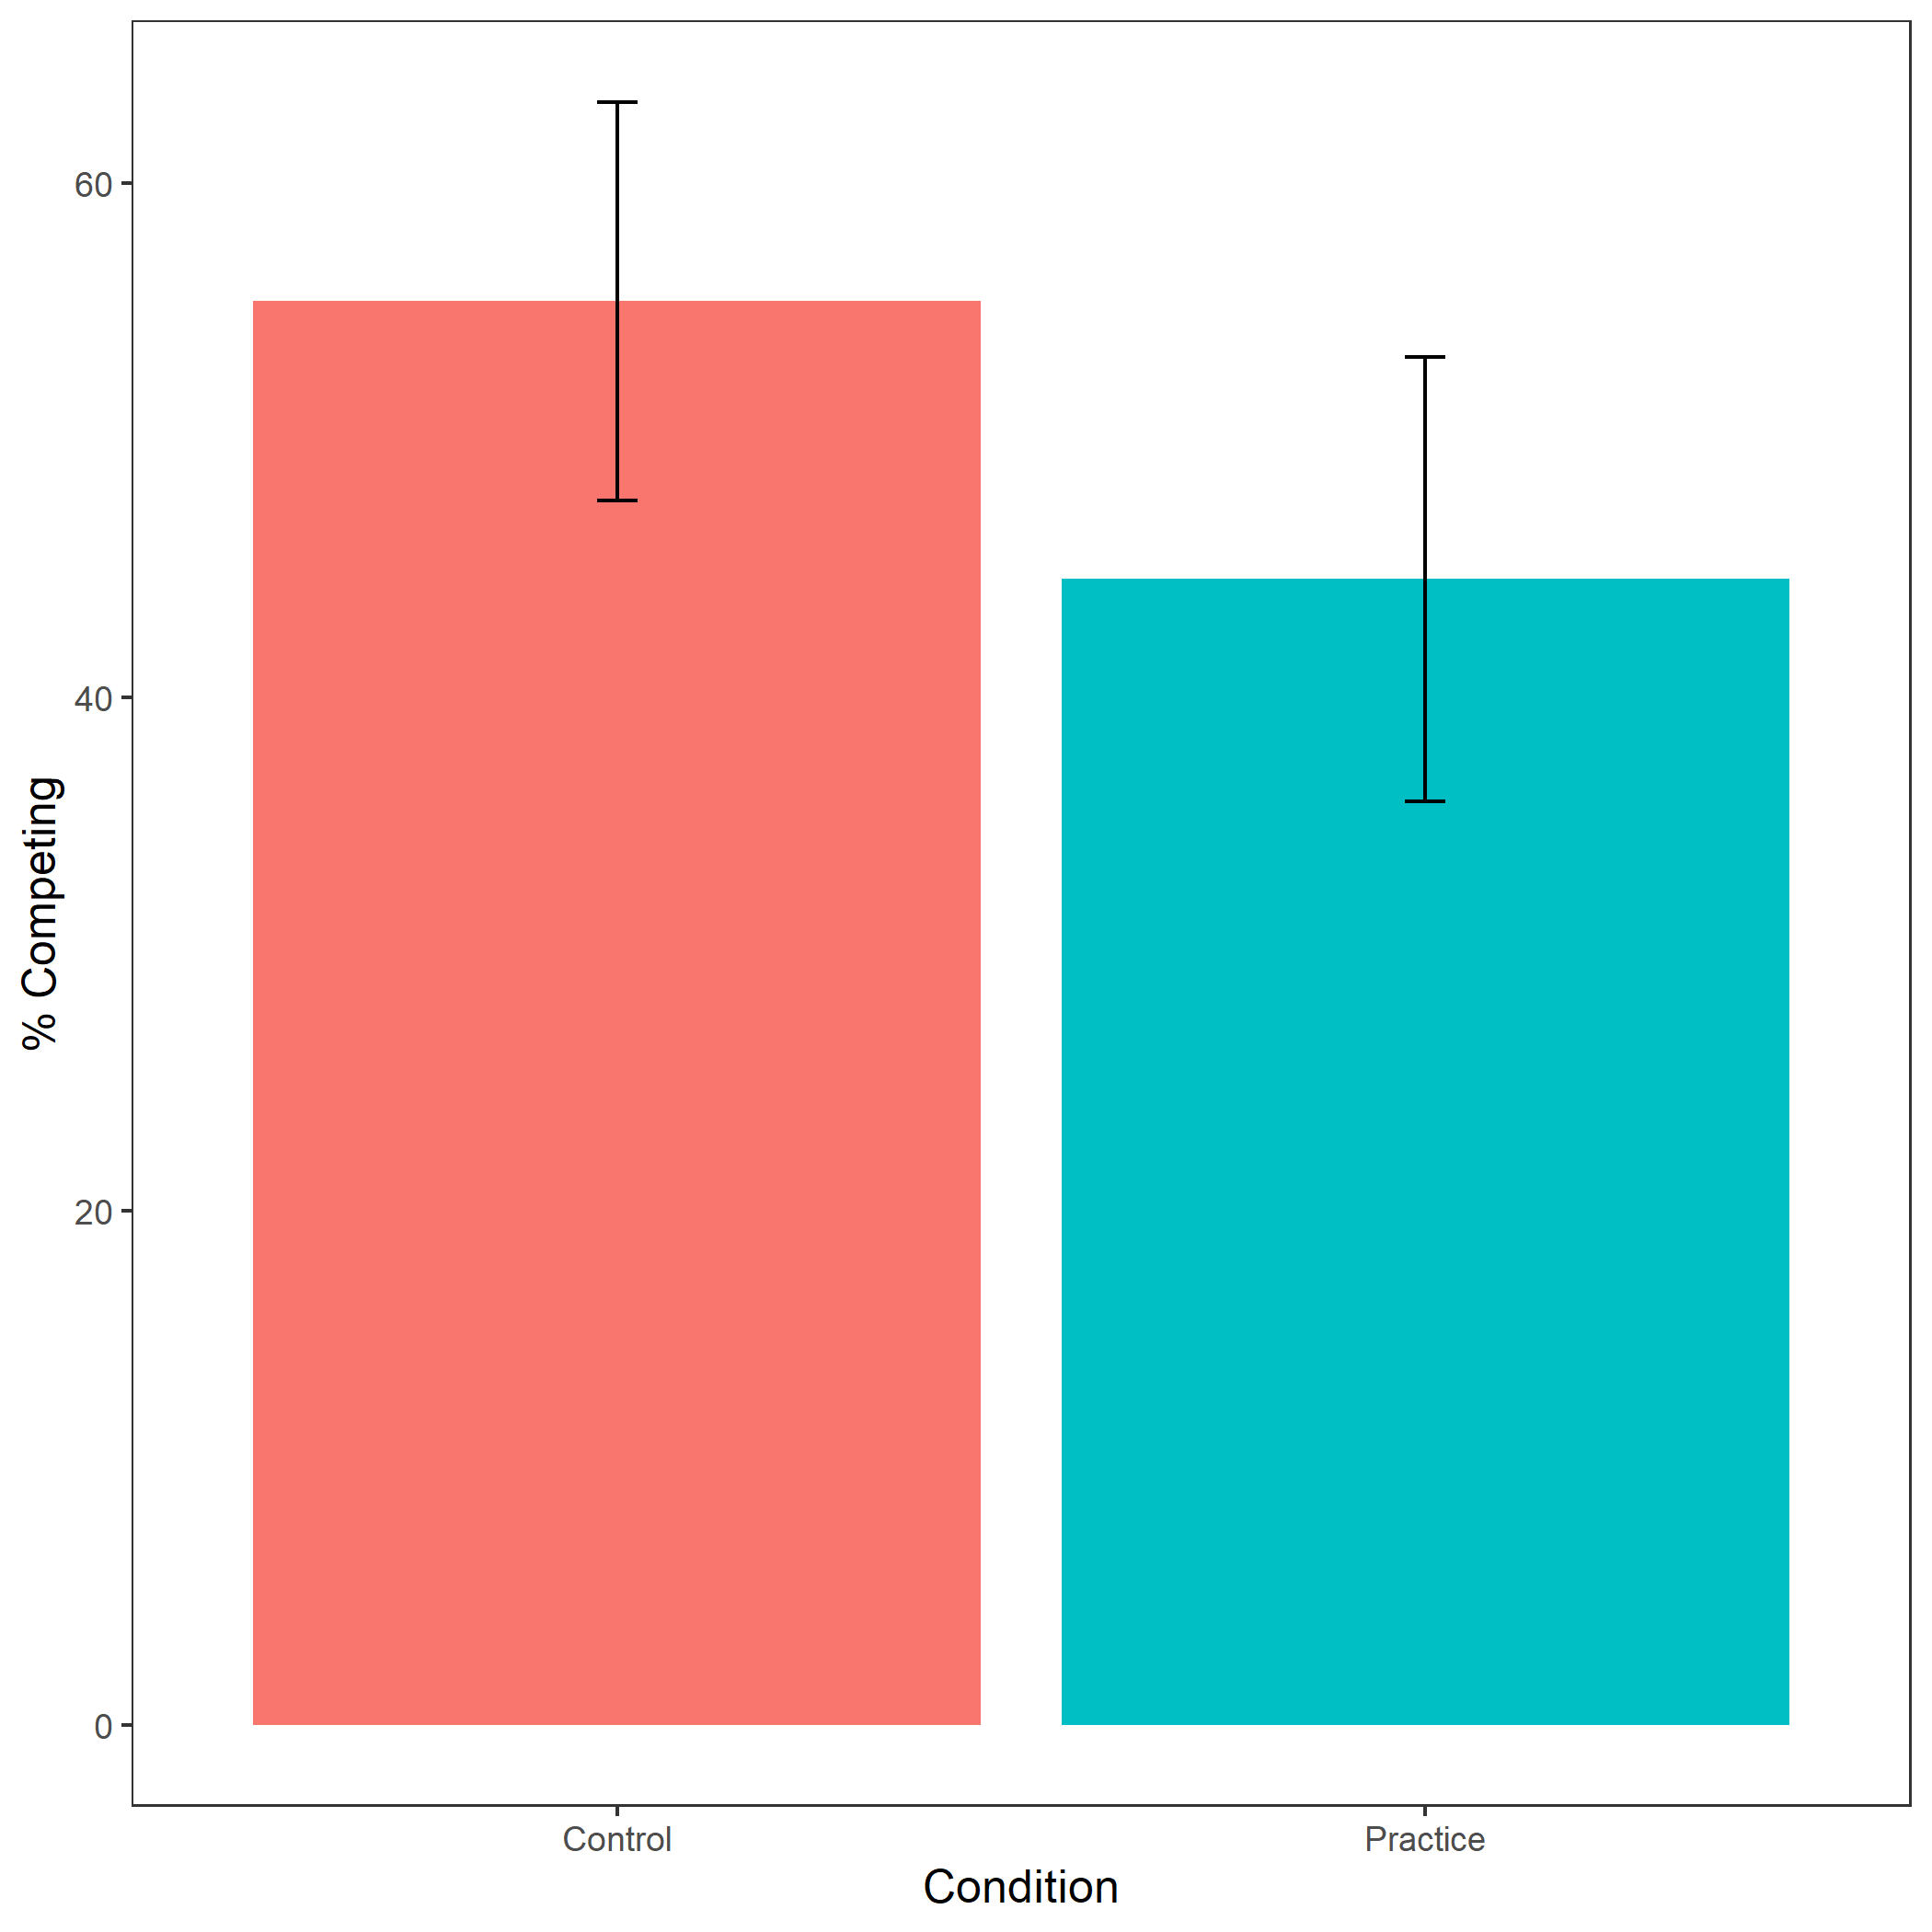
\includegraphics[width=29.17in]{C:/Users/keana/OneDrive - PennO365/Comp_transfer2018/Penn/practice_study/gender-practice/study2/figs/fig00_comp-choice-women-by-cond} \caption{Proportion of female participants who chose to compete by condition. We do not find evidence of the hypothesized effect of condition on the choice to compete, there were no significant differences in entry into competition between women in the control vs. prepare conditions. Error bars represent standard errors.}\label{fig:s200}
\end{figure}

\begin{figure}
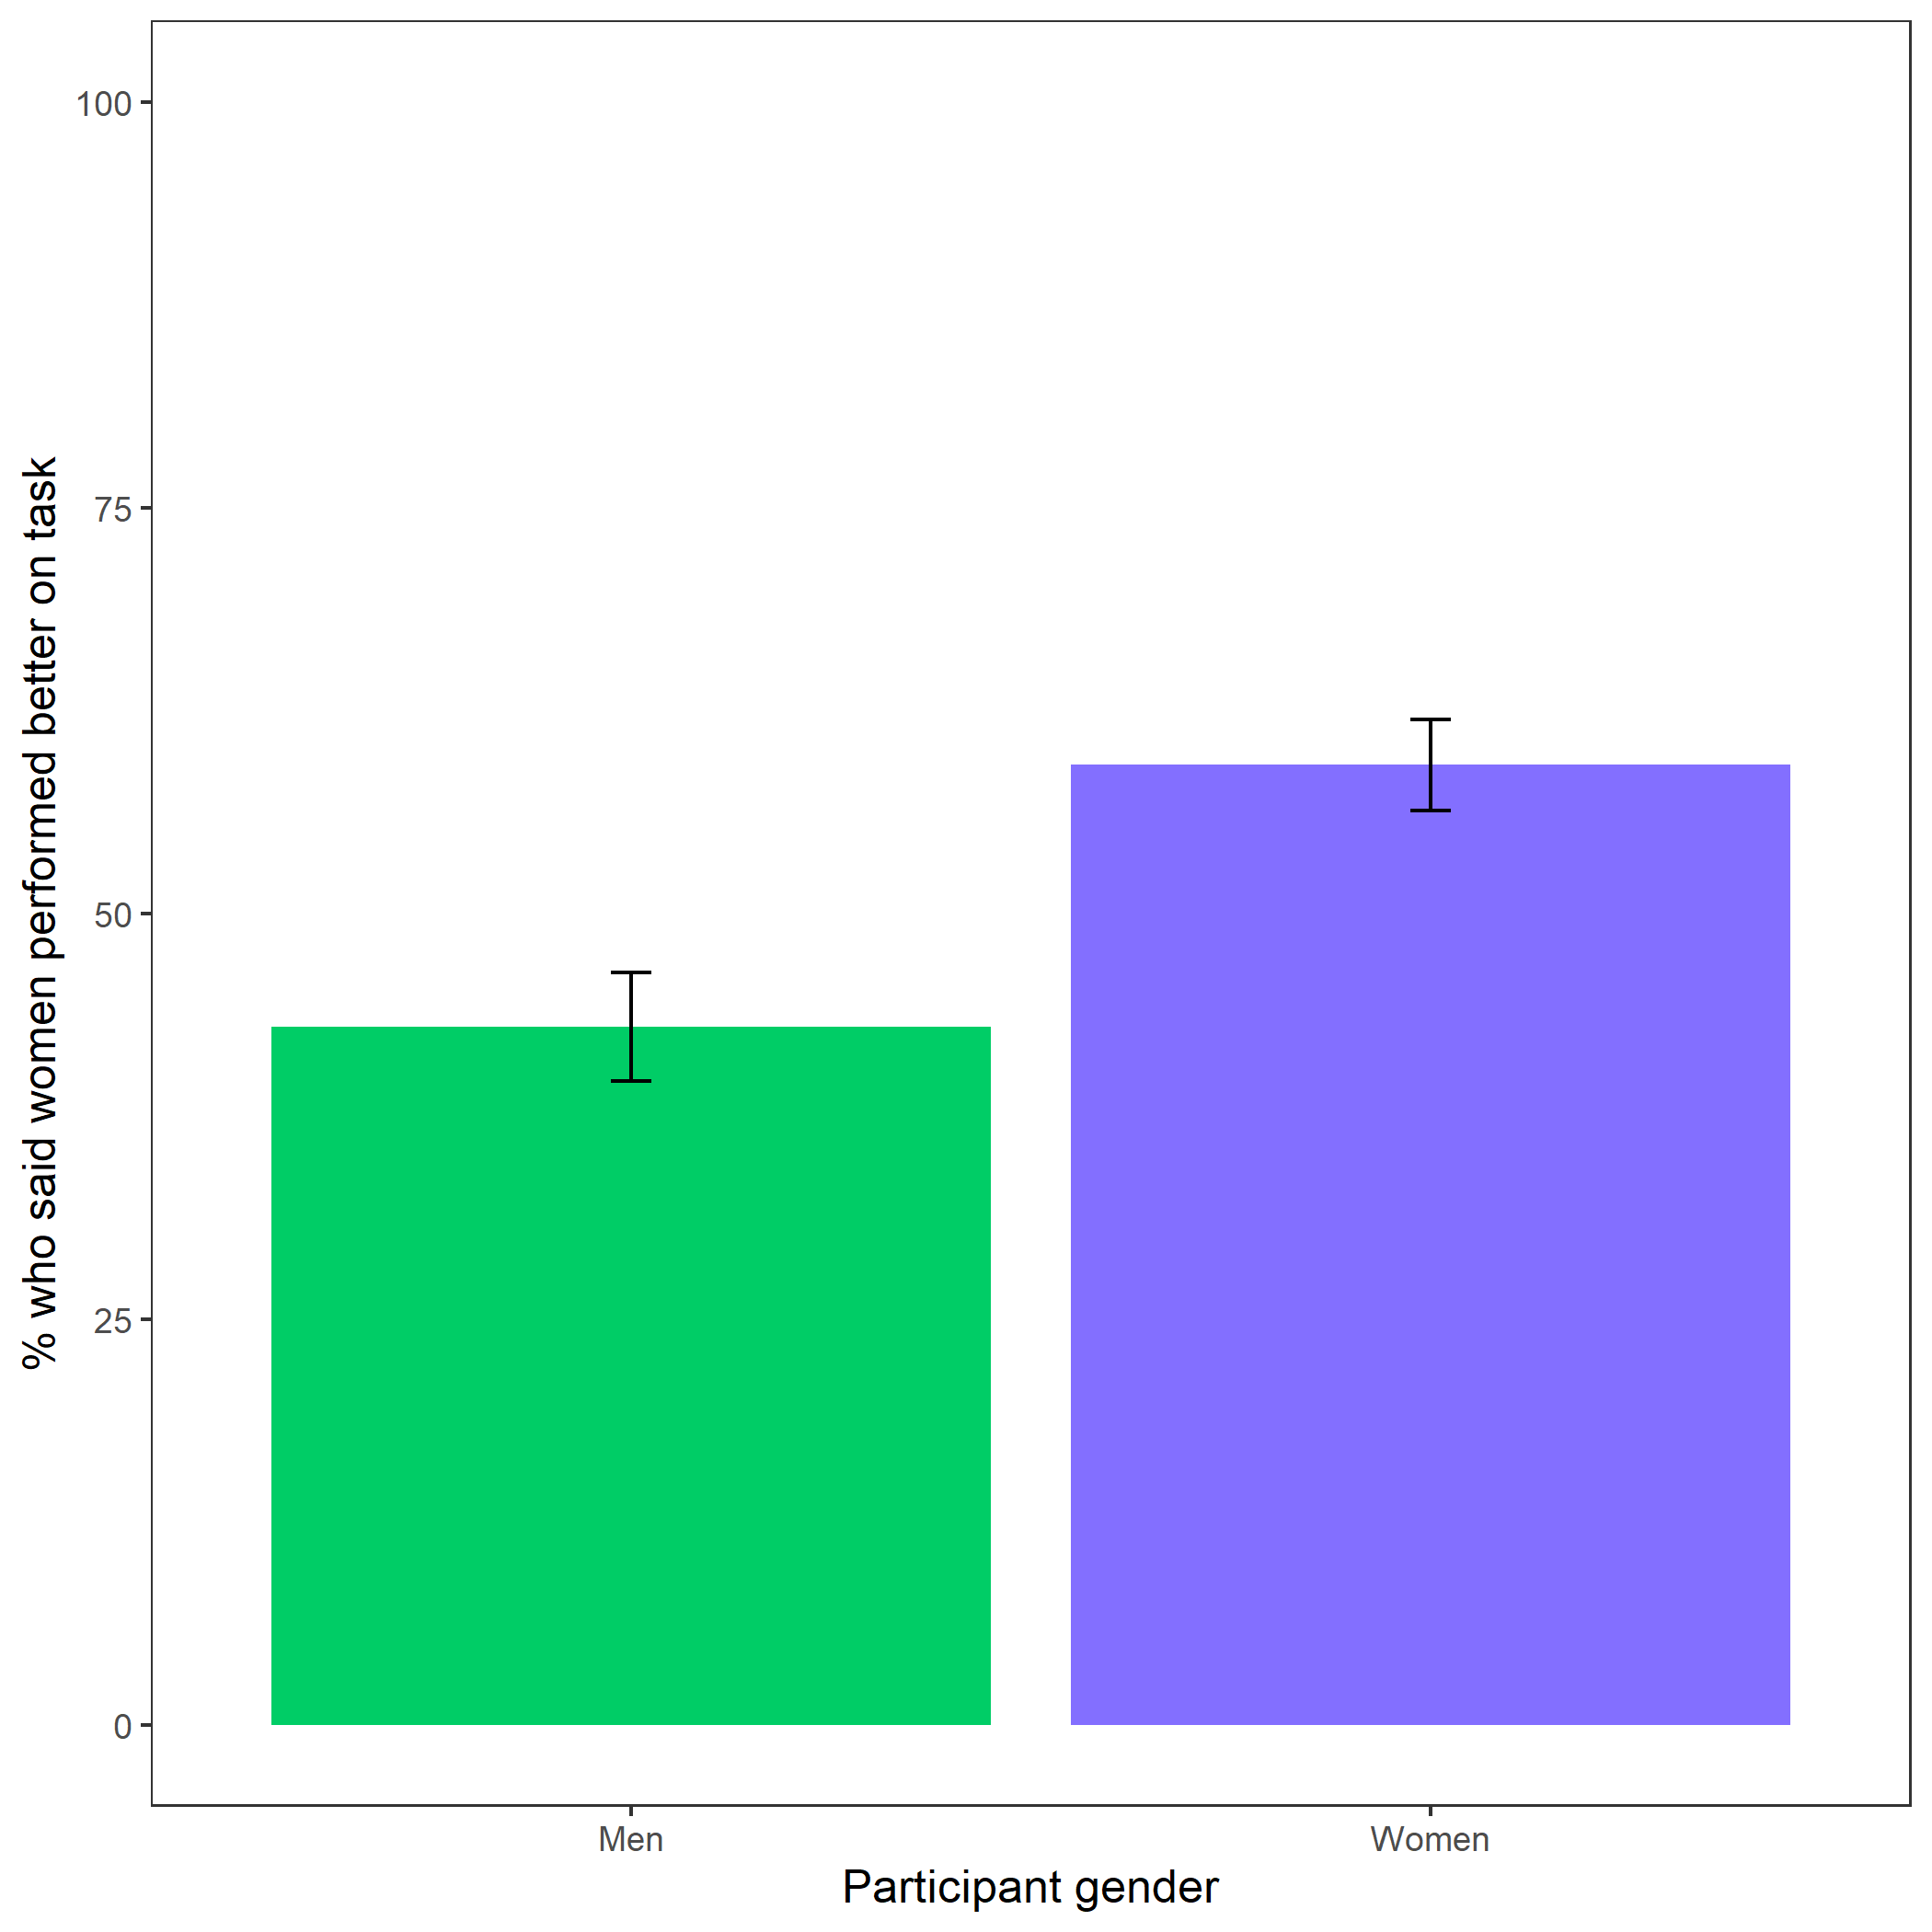
\includegraphics[width=29.17in]{C:/Users/keana/OneDrive - PennO365/Comp_transfer2018/Penn/practice_study/gender-practice/study2/figs/fig01_better-gender-guess} \caption{Participants' perceptions of gender differences in performance on the task. We replicate the effect from Study 1, where participants were not significantly more likely than chance to anticipate that one gender would perform better on the task. Error bars represent standard errors.}\label{fig:s201}
\end{figure}

\begin{figure}
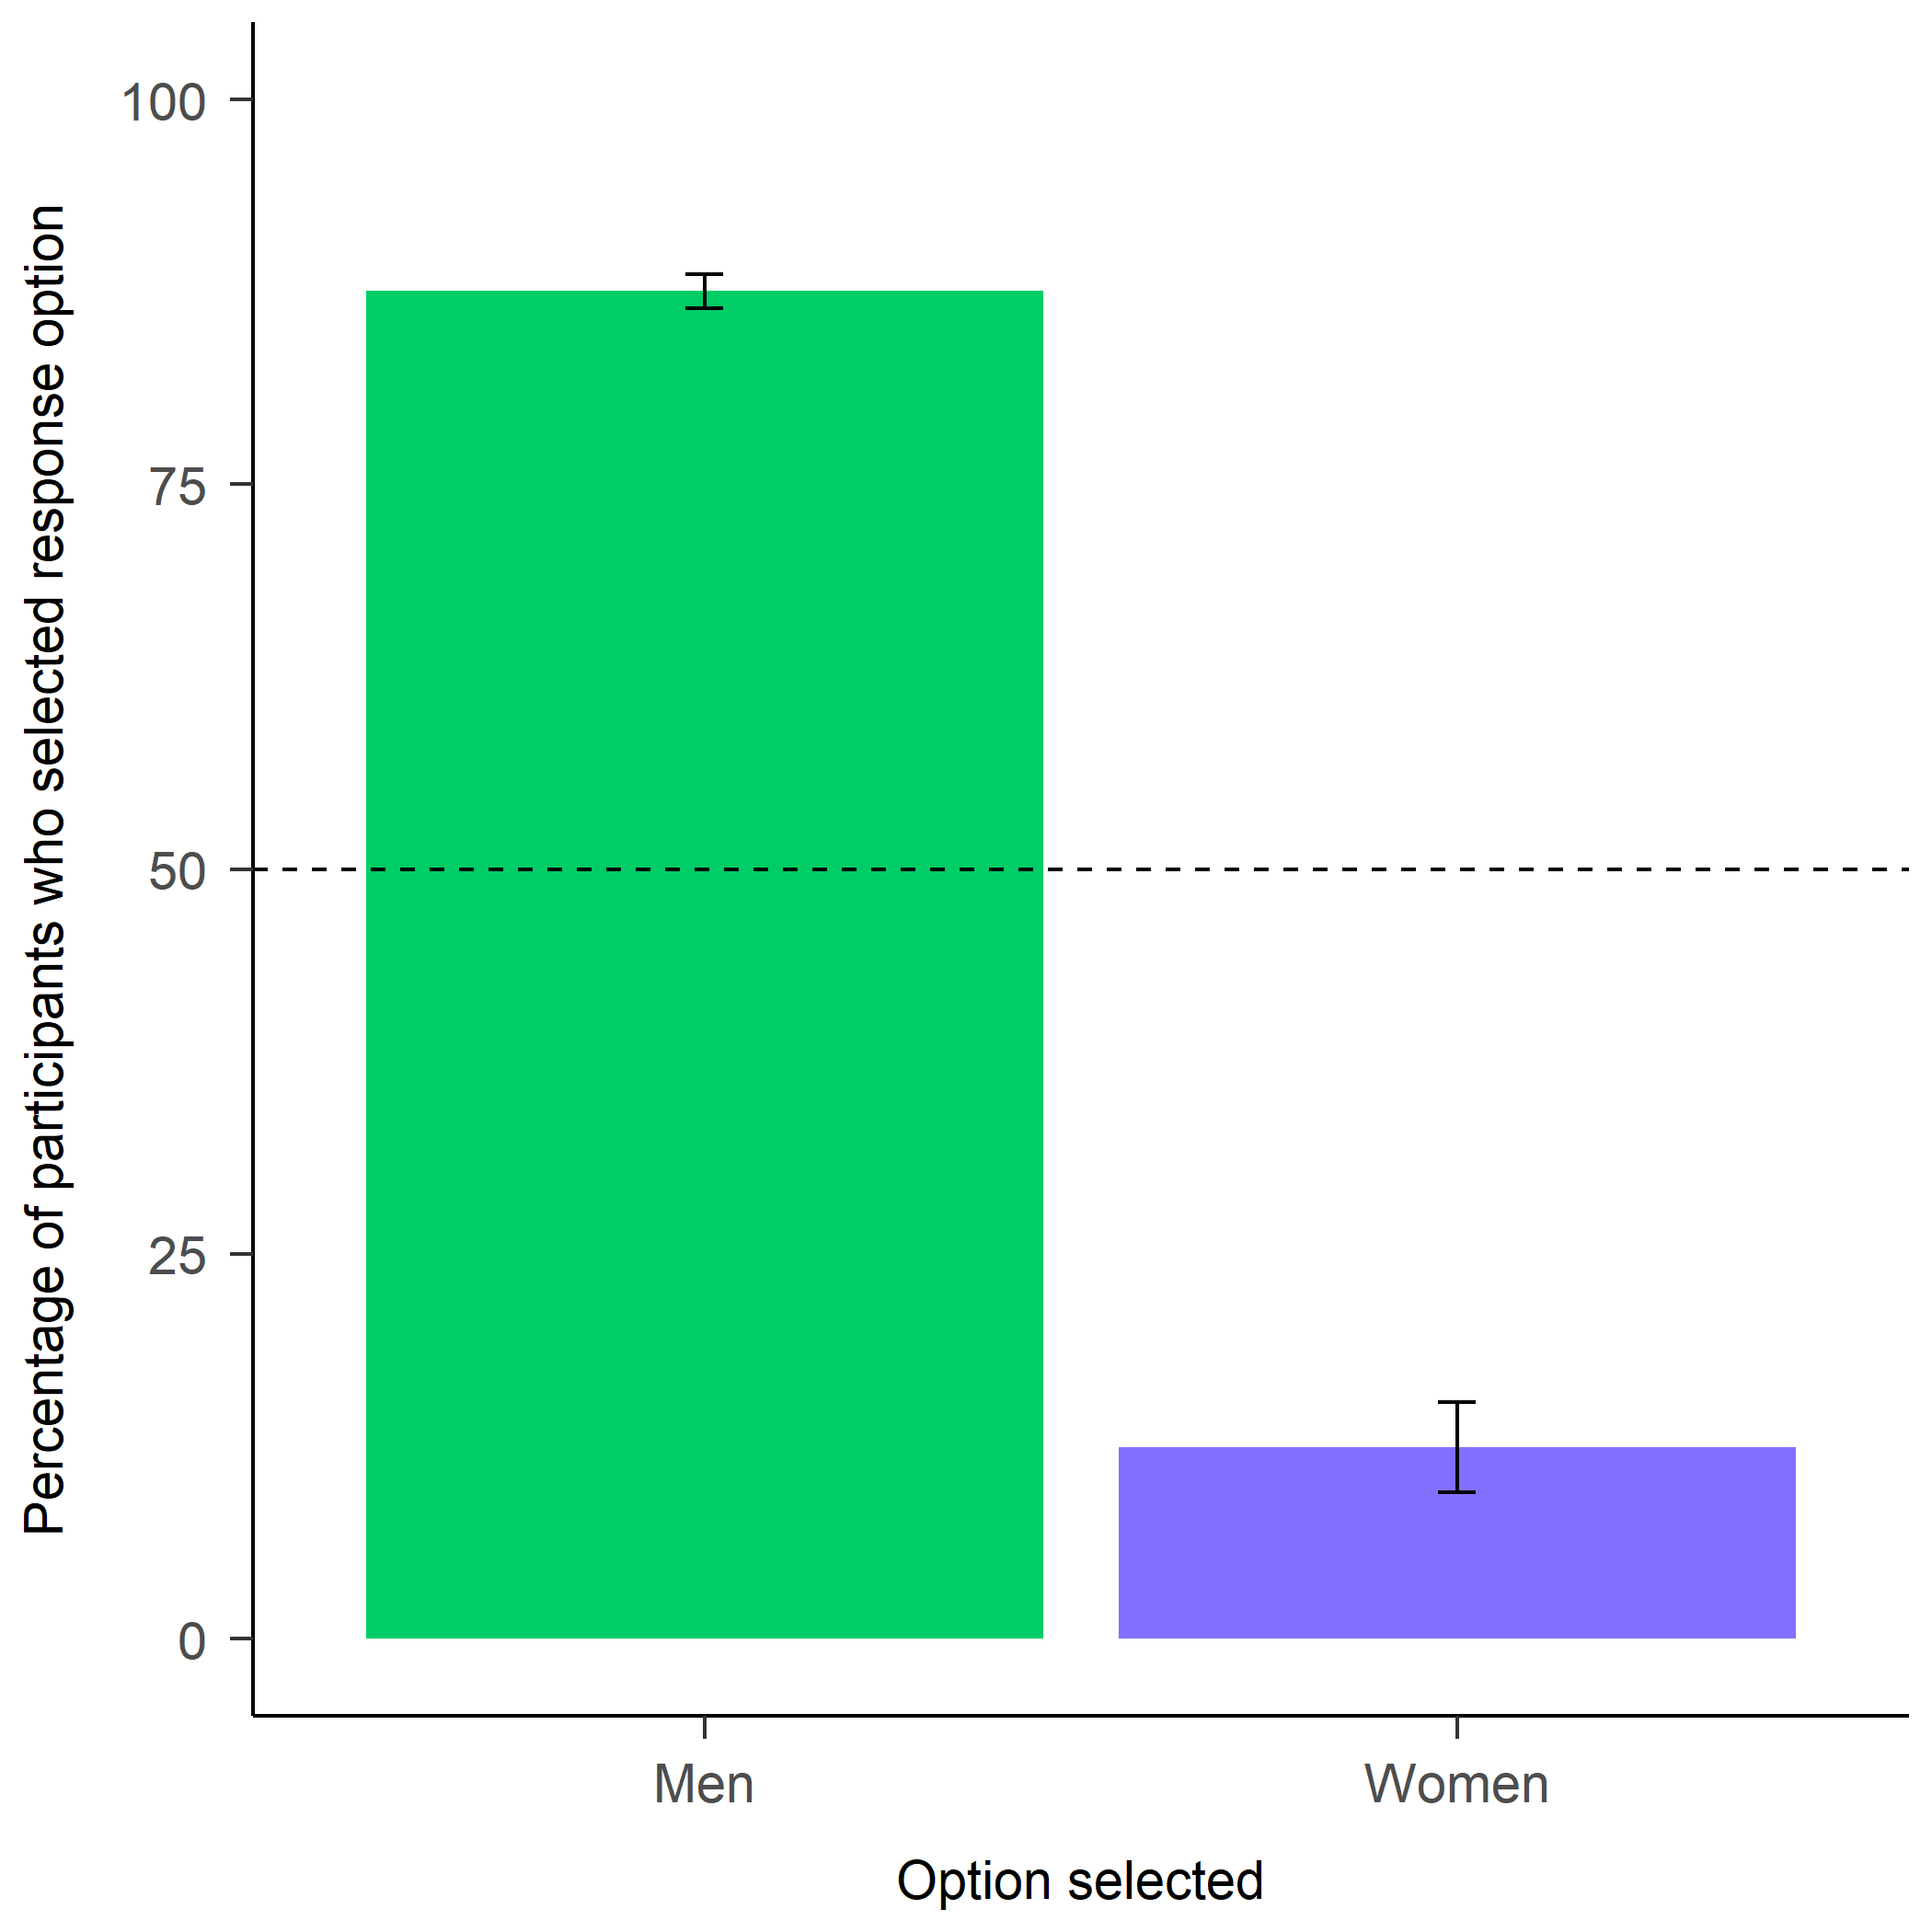
\includegraphics[width=29.17in]{C:/Users/keana/OneDrive - PennO365/Comp_transfer2018/Penn/practice_study/gender-practice/study2/figs/fig02_perc-gender-comp} \caption{Participants' perceptions of gender differences in choice to compete. Replicating the finding from Study 1, participants (especially men) in Study 2 are significantly more likely than chance to state that men chose the competitive payment scheme. Error bars represent standard errors.}\label{fig:s202}
\end{figure}

\begin{figure}
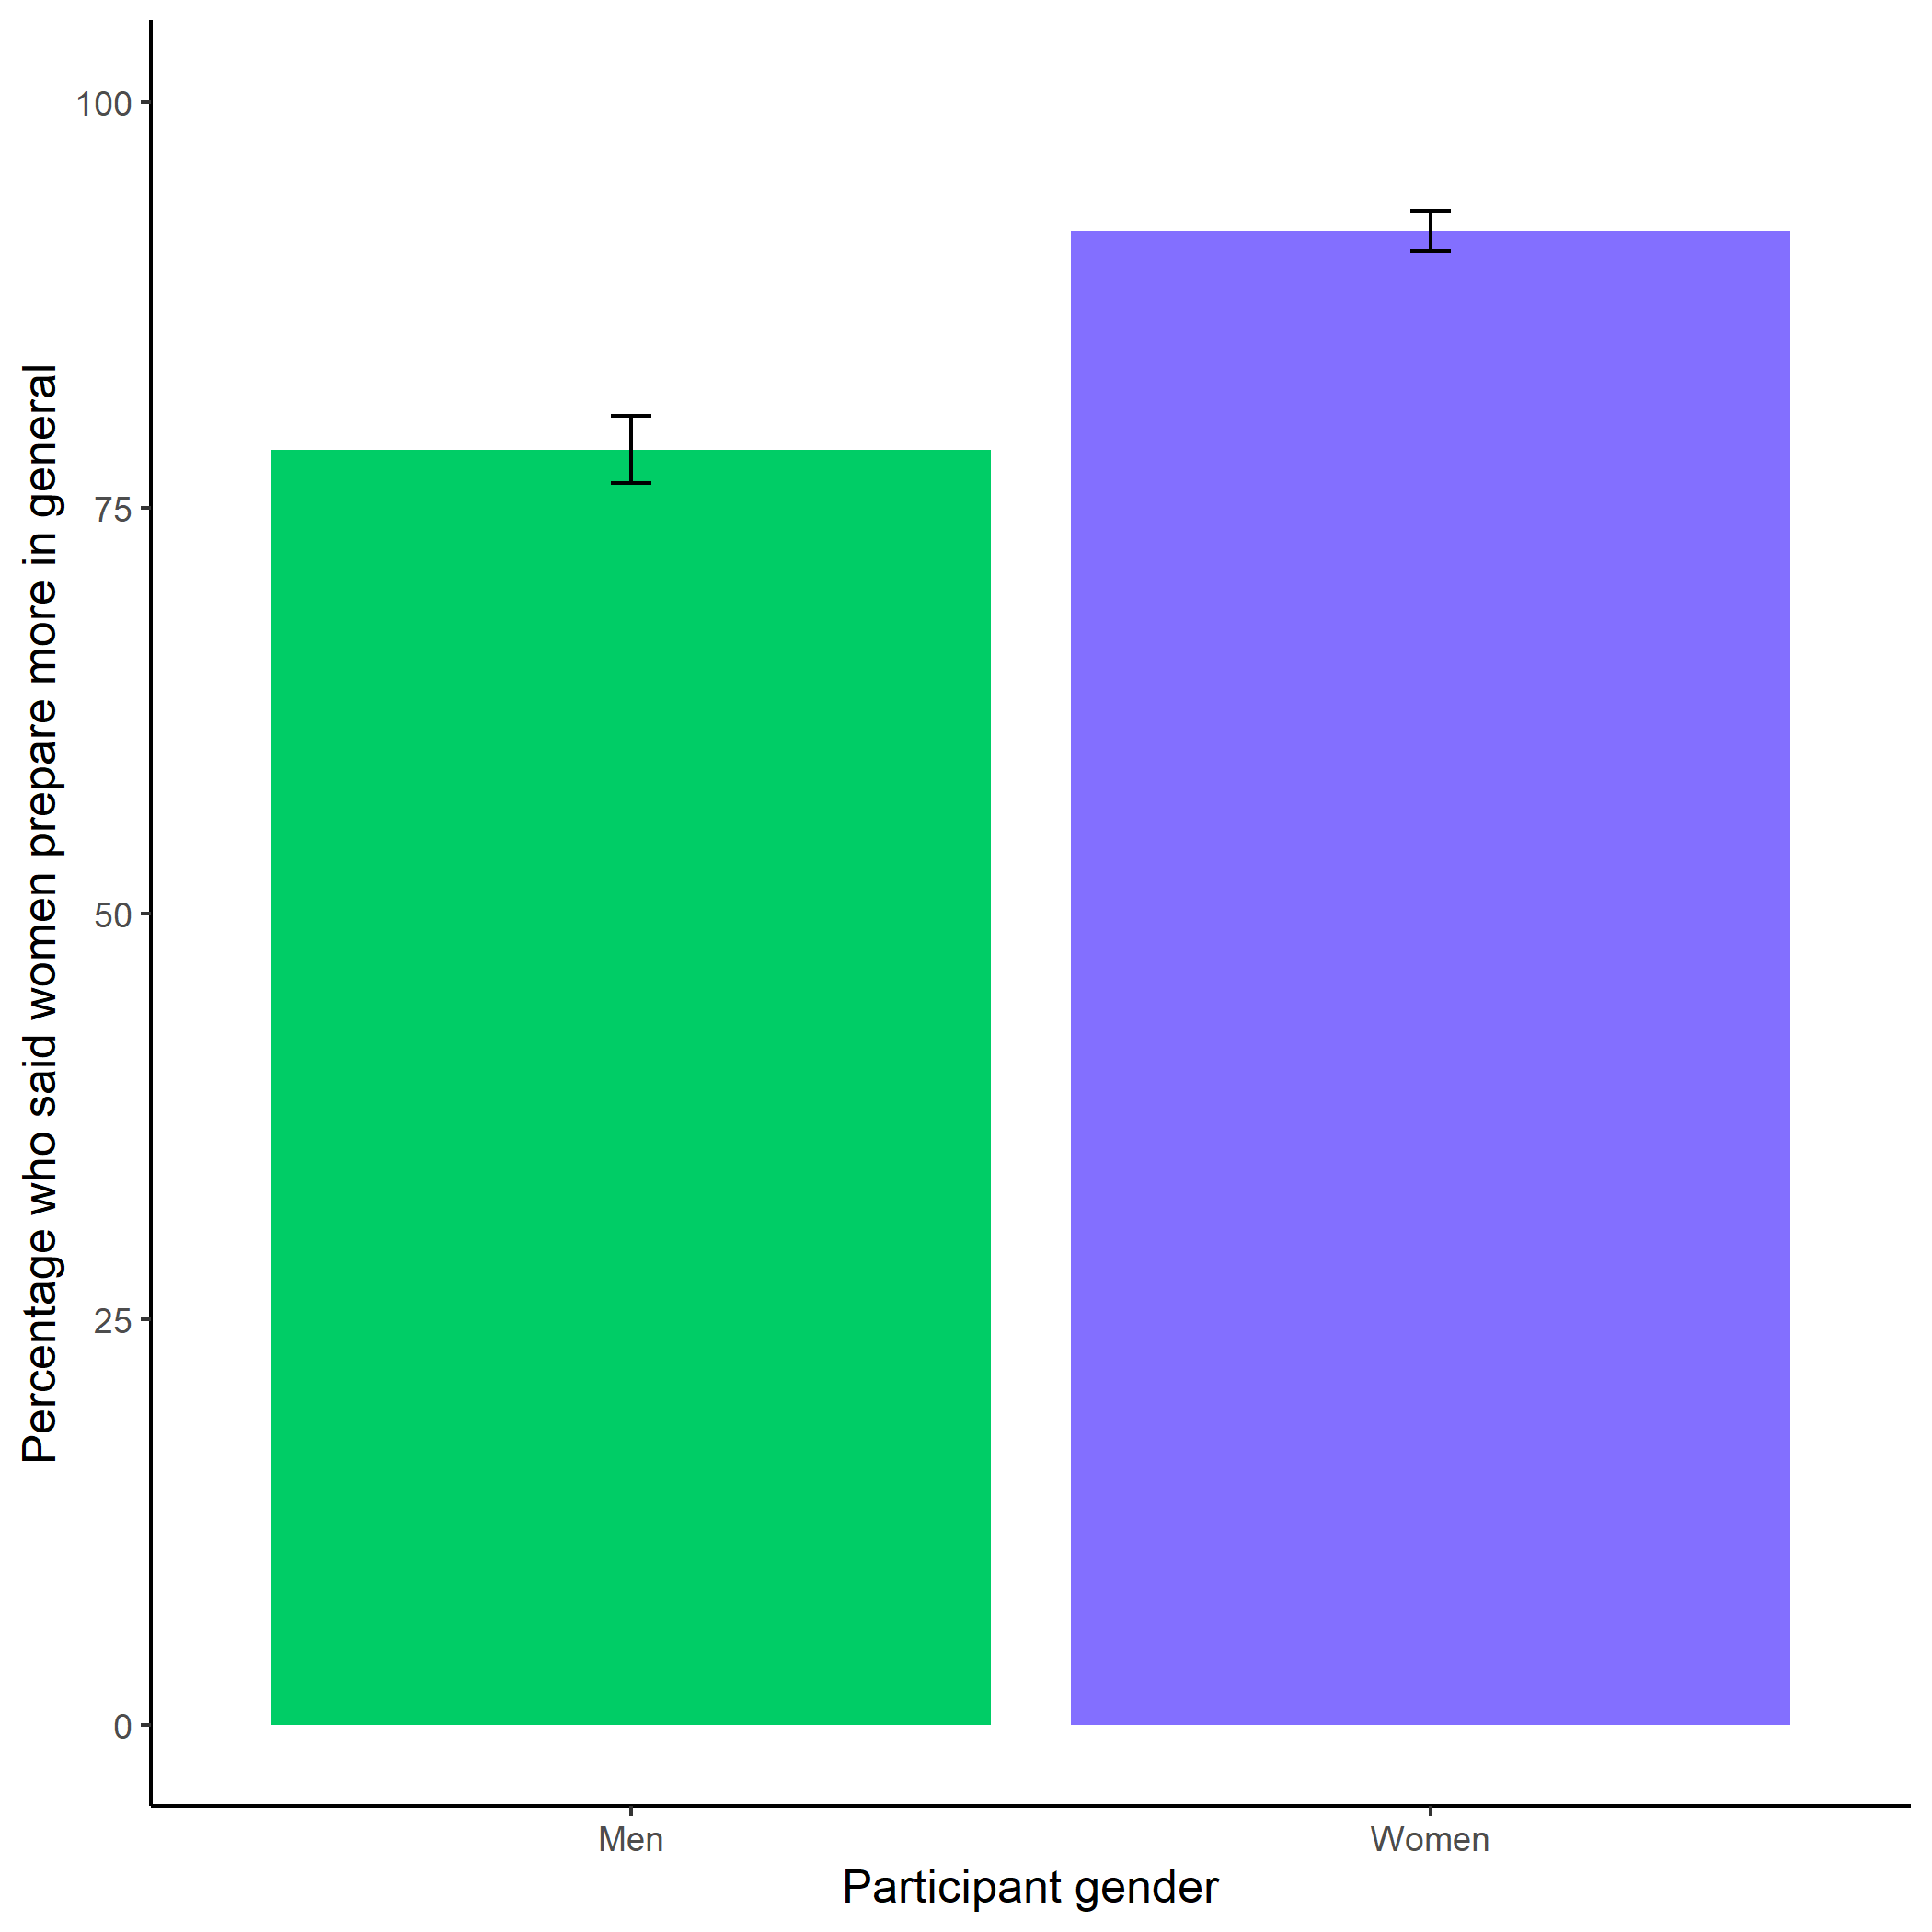
\includegraphics[width=29.17in]{C:/Users/keana/OneDrive - PennO365/Comp_transfer2018/Penn/practice_study/gender-practice/study2/figs/fig03_perc-gen-gender-pract} \caption{Participants' perceptions of general gender differences in choice to prepare. We replicate the findings from Study 1, where participants (especially women) are significantly more likely than chance to state that women prepare more in general than men. Error bars represent standard errors.}\label{fig:s203}
\end{figure}

\begin{figure}
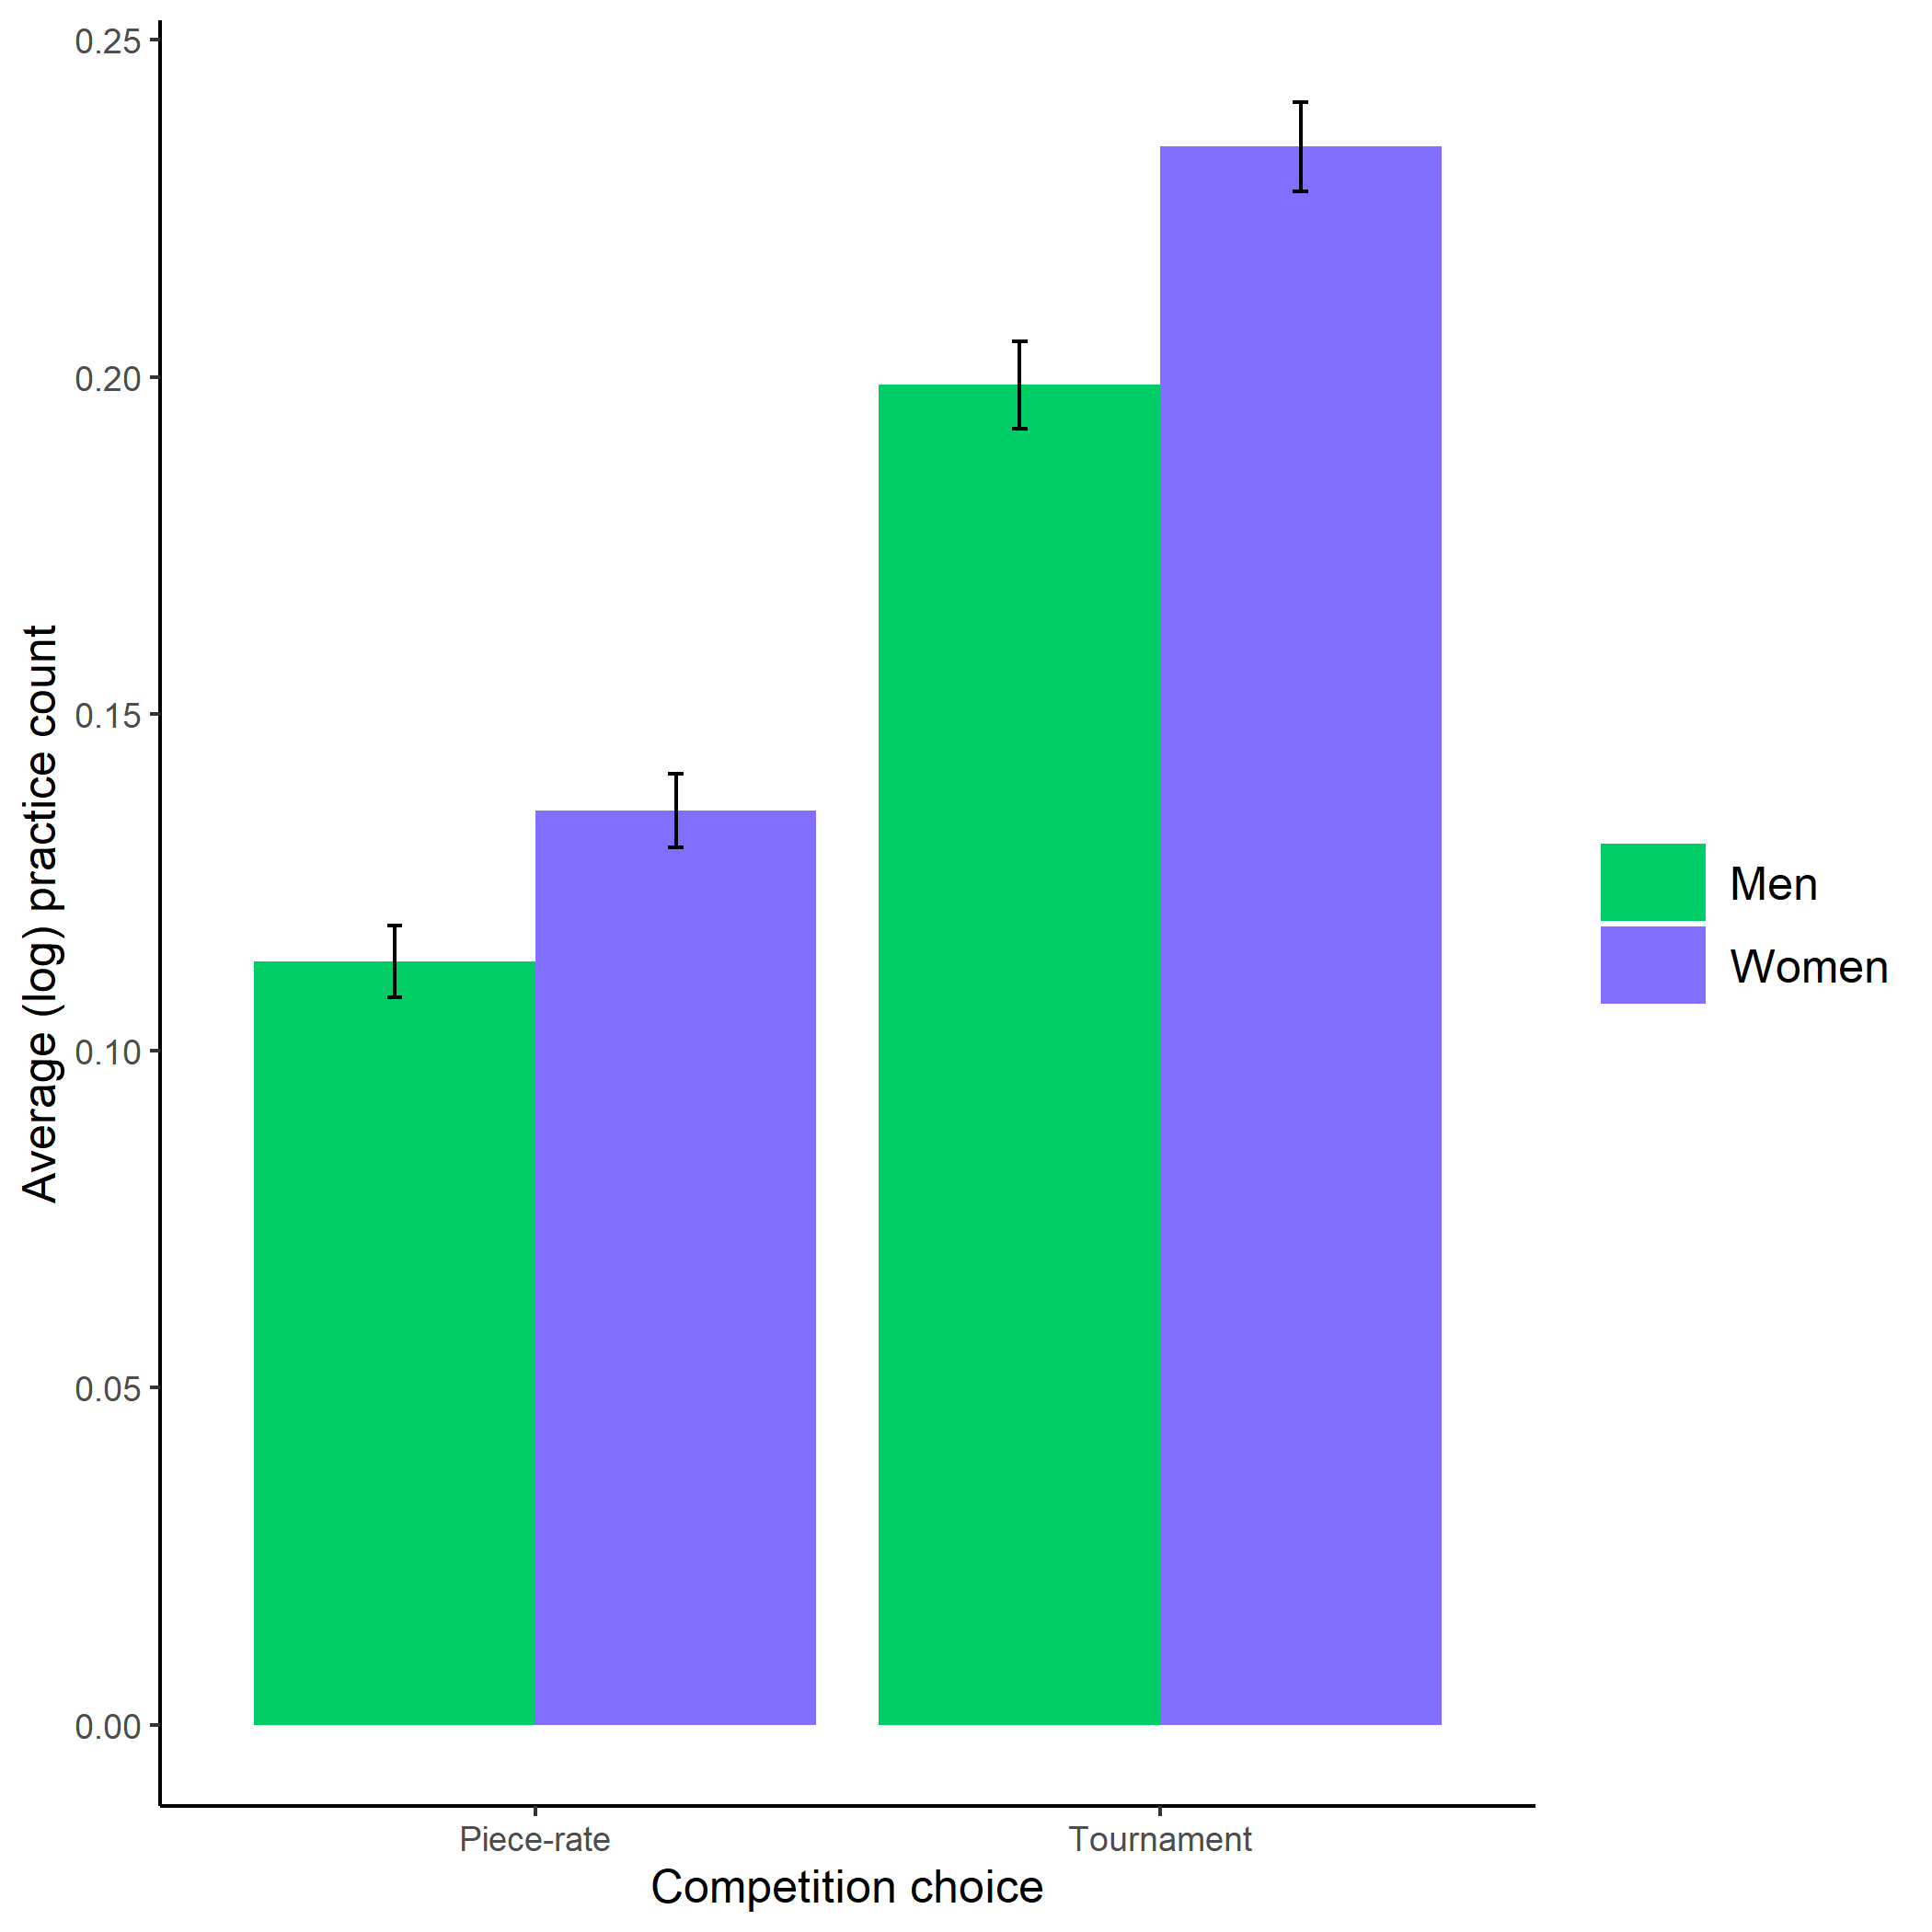
\includegraphics[width=29.17in]{C:/Users/keana/OneDrive - PennO365/Comp_transfer2018/Penn/practice_study/gender-practice/study2/figs/fig04_total-rev-count-by-gender-comp-choice} \caption{Gender differences in the number of extra preparation rounds chosen across participants' choice in a payment scheme. Here, we show that the gender gap in the choice to prepare is robust, even when half of the women are forced to prepare in the preparation condition. Error bars represent standard errors.}\label{fig:s204}
\end{figure}

\hypertarget{study-3}{%
\section{Study 3}\label{study-3}}

\startappendices

\hypertarget{the-first-appendix}{%
\chapter{The First Appendix}\label{the-first-appendix}}

This first appendix includes an R chunk that was hidden in the document (using \texttt{echo\ =\ FALSE}) to help with readibility:

\textbf{In 02-rmd-basics-code.Rmd}

\textbf{And here's another one from the same chapter, i.e.~Chapter \ref{code}:}

\hypertarget{the-second-appendix-for-fun}{%
\chapter{The Second Appendix, for Fun}\label{the-second-appendix-for-fun}}


%%%%% REFERENCES
\setlength{\baselineskip}{0pt} % JEM: Single-space References

{\renewcommand*\MakeUppercase[1]{#1}%
\printbibliography[heading=bibintoc,title={\bibtitle}]}


\end{document}
